% Created 2020-10-15 Thu 21:41
% Intended LaTeX compiler: pdflatex
\documentclass[11pt]{article}
\usepackage[utf8]{inputenc}
\usepackage[T1]{fontenc}
\usepackage{graphicx}
\usepackage{grffile}
\usepackage{longtable}
\usepackage{wrapfig}
\usepackage{rotating}
\usepackage[normalem]{ulem}
\usepackage{amsmath}
\usepackage{textcomp}
\usepackage{amssymb}
\usepackage{capt-of}
\usepackage{hyperref}
\usepackage{minted}
\IfFileExists{./resources/style.sty}{\usepackage{./resources/style}}{}
\IfFileExists{./resources/referencing.sty}{\usepackage{./resources/referencing}}{}
\addbibresource{./resources/references.bib}
\usepackage[mode=buildnew]{standalone}
\usepackage{tikz}
\usetikzlibrary{decorations.fractals}
\usetikzlibrary{lindenmayersystems}
\author{Ryan Greenup}
\date{\today}
\title{Page Rank}
\hypersetup{
 pdfauthor={Ryan Greenup},
 pdftitle={Page Rank},
 pdfkeywords={},
 pdfsubject={},
 pdfcreator={Emacs 27.1 (Org mode 9.4)}, 
 pdflang={English}}
\begin{document}

\maketitle
\tableofcontents



\section{Introduction}
\label{sec:org556b4af}
Any collection of interconnected information can form a network structure,
consider for example citations, webpages, wikis, power grids, wiring diagrams, encyclopedias and interpersonal
relationships. The analysis of these networks can be used to draw insights about
the behaviour of such networks.

One important form of analysis is \emph{netowork centrality}, a concept concerned with
the measure of the importance, popularity and relevance of a node. In a
relatively small graph, visualised in such a way so as to minimise the
overlapping of edges, a general expectation would be that the centrality score
would be correlated with geometric-centrality, this is demonstrated in figure
\ref{example-rs-graph} where the 2nd vertex has the highest \emph{PageRank} score and
is geometrically very central.

\subsection{The PageRank Method}
\label{sec:orgb84df95}

There are multiple ways to measure network centrality but this report is concerned with the \emph{PageRank} method, this method asserts that the centrality of a vertex can be
measured by the frequency of incidence with that vertex during a
random walk.

This approach only makes sense if the random walk can:

\begin{enumerate}
\item Traverse the entire network
\item Escape dead ends on a directed graph
\end{enumerate}


and so the \emph{PageRank} method involves:

\begin{itemize}
\item Altering a corresponding transition probability matrix such that it corresponds to a stochastic primitive \emph{Markov Chain}.
\item Considering the stationary distribution of this new graph.
\end{itemize}

\subsection{Power Walk and the Random Surfer}
\label{sec:org28de31a}
The typical method to adjust the transition probability matrix is the \emph{Random
Surfer}, introduced by Page and Brin in 1998
 \cite{larrypageAnatomyLargescaleHypertextual1998} as a distinguishing feature of
the \emph{Google} search engine, this aproach essentially introduces some probability
of teleporting to other nodes during a random walk, this is illustrated in
figure \ref{fig:rseg}.

A shortcoming of this approach is that it assumes all edges are positively weighted. This
menas that the model treats any link as an endorsement of the destination
node, this may not necessarily always be true (consider for exmple burned-in
advertisements or negative reviews). In the past attributing weights to links was not particularly feasible, recent developments in sentiment analysis has however made this possible meaning that this limitation is more significant.

The \emph{Power Walk} approach, introduced by Park and Simoff in 2013 \cite{parkPowerWalkRevisiting2013} is an alternative way to create a transition
probability matrix that is defined for real weighted edges and could be used with sentiment analysis to more effectively measure network centrality.

These individual appraches are discussed in more detail at \ref{PageRank-Generally}.

\subsection{Stability and Convergence}
\label{sec:orgd6359eb}

The rate at which the algorithm for \emph{PageRank} converges to a solution and the stability of that solution can both be measured by the second eigenvalue of the corresponding transition probability matrix (The details of this are discussed at \ref{second-eigenvalue}).

It is not clear how the second eigenvalue is related to the method parameters of the \emph{Power Walk} algorithm \cite[\textsection 3.4]{parkPowerWalkRevisiting2013} and this report aims to:

\begin{enumerate}
\item Implement methods to perform \emph{PageRank} analysis using:
\begin{enumerate}
\item The \emph{Random Surfer} model
\item The \emph{Power Walk} model
\end{enumerate}
\item Investigate the Relationship between the parameters of the \emph{Power Walk}
transition probability matrix and the second eigenvalue
\end{enumerate}

\part{Implementing PageRank}
\section{Mathematics of Page Rank}
\label{PageRank-Generally}
\subsection{The Stationary Distribution of a Probability Transition Matrix}
\label{sec:orgf855ea4}
A graph can be expressed as an adjacency matrix \(\mathbf{A}\):

\[
A_{i,j} \in \left\{ 0,1 \right\}
\]

Where each element of the matrix indicates whether or not travel from
vertex \(j\) to vertex \(i\) is possible with a value of 1. \footnote{Some
authors define an adjacency matrix transposed (see e.g.
\cite{rosenDiscreteMathematicsIts2007,AdjacencyMatrix2020a,meghabghabSearchEnginesLink2008})
this unfourtunately includes the \texttt{igraph} library
\cite{gaborcsardiIgraphManualPages2019} but that convention will not be
followed in this paper}

During a random walk the probability of arriving at vertex \(j\) from vertex
\(i\) can similarly be described as an element of a transition probability
matrix \(\mathbf{T}_{i,j}\), this matrix can be described by the following
relationship \footnote{In this paper \(\vec{1}\) refers to a vector containing only
values of 1, the size of which should be clear from the context}:

\begin{align}
\mathbf{T} &= \mathbf{A} \mathbf{D}^{-1}_{\mathbf{A}} \label{eq:basic-trans-def} : \\
& \mathbf{D}_{\mathbf{A}} = \mathrm{diag}\left(\vec{1} \mathbf{A}\right) \label{eq:diagScaleDef}
\end{align}

The value of \(\mathbf{D}\) is such that under matrix multiplication
\(\mathbf{A}\) will have columns that sum to 1 (i.e. a \emph{column
stochastic matrix}, see \textsection \ref{definitions}), for a reducible
or non-stochastic graph the definition of \(\mathbf{D}\) would need to
be adjusted to acheive this, this is discussed below 

During the random walk, the running tally of frequencies, at the
\(i^{\mathrm{th}}\) step of the walk, can be described by a vector
\(\vec{p}\), this vector can be determined for each step by matrix
multiplication:

\begin{align}
\vec{p_{i+1}} = \mathbf{T}\vec{p_{i}} \label{eq:recurrence}
\end{align}

This relationship is a linear recurrence relation, more importantly
however it is a \emph{Markov Chain}
\cite[\textsection 4.4]{langvilleGooglePageRankScience2012}.

Finding the Stationary point for this relationship will give a
frequency distribution for the nodes and a metric to measure the
centrality of vertices.

\subsection{Random Surfer Model}
\label{sec:org33c0829}
\subsubsection{Problems with the Stationary Distribution}
\label{issues}
The approach in \ref{PageRank-Generally} has the following issues

\begin{enumerate}
\item Convergence of \eqref{eq:recurrence}
\begin{enumerate}
\item Will this relationship converge or diverge?
\item How quickly will it converge?
\item Will it converge uniquely?
\end{enumerate}
\item Reducible graphs
\begin{enumerate}
\item If it is not possible to perform a random walk across an entire graph for all initial conditions, this approach doesn't have a clear analogue.
\end{enumerate}
\item Cycles
\begin{enumerate}
\item A graph that is cyclical may not converge uniquely
\begin{enumerate}
\item Consider for example the graph \(A\rightarrow B\).
\end{enumerate}
\end{enumerate}
\end{enumerate}

\subsubsection{Markov Chains}
\label{markov}
The relationship in \eqref{eq:recurrence} is a \emph{Markov Chain}  and it is known
that the power method will converge: \footnote{A \emph{Markov Chain} is
simply any process that evolves depending on it's current condition, it's
interesting to note however that the theory of \emph{Markov Chains} is not mentioned in any
of the original papers by page and brin
\cite[\textsection 4.4]{langvilleGooglePageRankScience2012}}

\begin{itemize}
\item for a stochastic irreducible markov chain \cite[\textsection 1.5.5]{larsonElementaryLinearAlgebra1991},
\item regardless of the initial condition of the process for an \emph{aperiodic} Markov chain \cite[\textsection 4.4]{langvilleGooglePageRankScience2012}
\end{itemize}

\paragraph{Stochastic}
\label{stochastic}
If a vertex had a 0 outdegree the corresponding column sum for the adjacency
matrix describing that graph would also be zero and the matrix non-stochastic,
this could occur in the context of a random walk where a link to a page with no
outgoing links was followed (e.g. an image), this would be the end of the
walk.

So to ensure that \eqref{eq:recurrence} will converge, the probability transition
matrix must be made stochastic, to acheive this a uniform probability of teleporing from a dead end to any other vertex can be introduced:

\begin{align}
\mathrm{S} = \mathrm{T}+ \frac{\vec{a} \cdot \vec{1}^{\mathrm{T}} }{n} \label{eq:nearly-random-surfer}
\end{align}

This however would not be sufficient to ensure that \eqref{eq:recurrence} would converge, in addition the transition probability matrix must be made irreducible and aperiodic (i.e. primitive). \cite{langvilleGooglePageRankScience2012}

\begin{figure}[htbp]
\centering
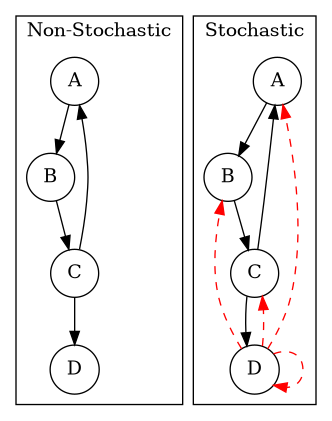
\includegraphics[width=6cm]{media/dot/stochastic_graph_example.dot.png}
\caption{\label{fig:stochastic-example}\(D\) is a \emph{dangling node}, a dead end during a random walk, the corresponding probability transition matrix \((\mathbf{T})\) is hence non-stochastic (and also reducible), Introducing some probability of teleporting from a dead end to any other vertex as per \eqref{eq:nearly-random-surfer} (denoted in red) will cause \(\mathbf{T}\) to be stochastic.}
\end{figure}

\paragraph{Irreducible}
\label{sec:orge2b85b1}
A graph that allows travel from any given vertex to any other vertex is said to be irreducible \cite{langvilleGooglePageRankScience2012}, see for example figure \ref{irreducible-example}, this is important in the context of a random walk because only in an irreducible graph can all vertexes be reached from any initial condition.

\begin{figure}[htbp]
\centering
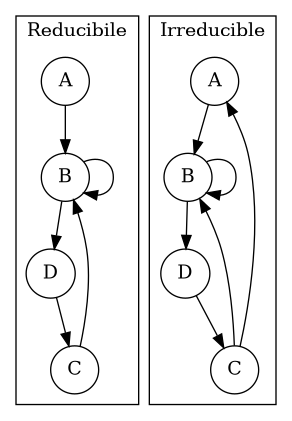
\includegraphics[width=6cm]{media/dot/reducible_graph_example.dot.png}
\caption{\label{irreducible-example}Example of a reducible graph, observe that although \(C\) is not a dead end as discussed in \ref{stochastic}, there is no way to travel from \(C\) to \(A\), by adding an edge such an edge in the resulting graph is irreducible. The resulting graph is also aperiodic (due to the loop on \(B\)) and stochastic, so there will be a stationary distribution corresponding to \eqref{eq:recurrence}.}
\end{figure}

\paragraph{Aperiodic}
\label{sec:org82c8a83}
An a periodic graph has only one eigenvalue that lies on the unit circle, this is important because \(\lim_{k\rightarrow \infty} \left( \frac{\mathbf{A}}{r}^{k} \right)\) exists for a non-negative irreducible matrix \(\mathbf{A}\) if and only if \mathbf{A} is aperiodic. A graph that is a periodic can be made aperiodic by interlinking nodes \footnote{Actually it would be sufficient to merely link one vertex to itself \cite[\textsection 15.2]{langvilleGooglePageRankScience2012} but this isn't very illustrative or helpful in this context}


\begin{figure}[htbp]
\centering
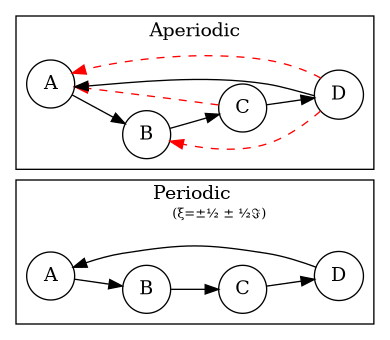
\includegraphics[width=9cm]{media/dot/aperiodic.dot.png}
\caption{\label{fig:aperiodic}A periodic graph with all eigenvalues on the unit circle \(\xi = \frac{\sqrt{2}}{2} e^{\frac{\pi i}{4} k}\), by adding in extra edges the graph is now aperiodic, this does not represent the random surfer model, which would in theory connect every vertex but with some probability.}
\end{figure}

\paragraph{The Fix}
\label{fix}
To ensure that the transition probability matrix is primitive (i.e. irreducible and aperiodic) as well as stochastic, instead of introducing the possible to teleport out of dead ends, introduce a probability of teleporting to any node at any time (\(\alpha\)), this approach is known as the \emph{Random Surfer} model and the transition probability matrix is given by \cite{larrypageAnatomyLargescaleHypertextual1998} :

\begin{align}
\mathbf{S} = \alpha \mathbf{T} + \frac{(1- \alpha)}{n} \mathbf{J} \label{eq:random-surfer}
\end{align}

This matrix is primitive and stochastic and so will converge (it is also unfourtunately completely dense, see \ref{solving-stationary-dist} \cite[\textsection 4.5]{langvilleGooglePageRankScience2012}.

The relation ship in \eqref{eq:recurrence} can now be re expressed as:

\begin{align}
\vec{p_{i+1}} \rightarrow \mathbf{T} \vec{p}_{i} \label{eq:random-surfer-recurrence}
\end{align}



\begin{figure}[htbp]
\centering
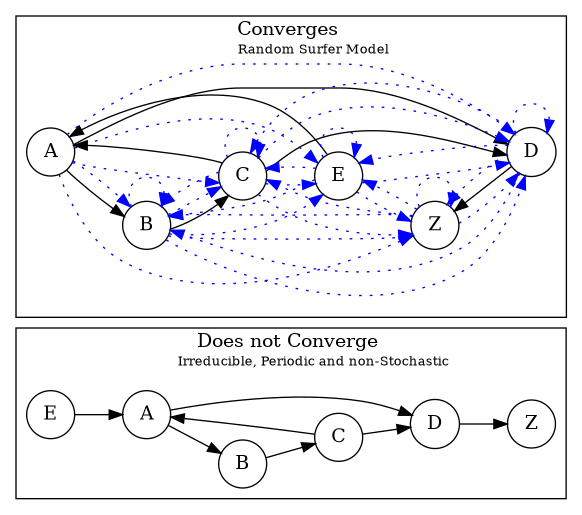
\includegraphics[width=9cm]{media/dot/random_surfer.dot.png}
\caption{\label{fig:rseg}A graph that is aperiodic, reducible and non-stochastic, by applying the random surfer model \eqref{eq:random-surfer} blue \emph{teleportation} edges are introduced, these may be followed with a probability of \(1 - \alpha\)}
\end{figure}
\subsubsection{Limitations}
\label{sec:orgacab0f9}
The \emph{Random Surfer} Model can only consider positively weighted edges, it cannot
take into account negatively weighted edges. This limitation is increasingly
important as techniques of sentiment analysis are developed which could indicate
that links promote aversion rather than endorsement (e.g. a negative review or
an innapropriate advertisement).
\subsection{Power walk}
\label{pwalk}
The \emph{Power Walk} method is an alternative approach to develop a probability
transition matrix to use in place of \eqref{eq:recurrence}.

Let the probability of travelling to a non-adjacent vertex be some value \(x\)
and \(\beta\) be the ratio of probability between following an edge or
teleporting to another vertex.

This transition probability matrix would be such that the probability of
travelling some vertex \(j \rightarrow i\) would be :

\begin{align}
\mathbf{W}_{i, j} = x\beta^{\mathbf{A_{i,j}}} \label{eq:prob-power-walk}
\end{align}

Where \(\mathbf{W}\) denotes the power walk probability transition matrix.

Whe probability of travelling to any given vertex must be 1 and so:


\begin{align}
      1 &= \sum^{n}_{j= 1}   \left[ x \beta^{\mathbf{A_{i,j}}} \right] \\
       \implies  x&= \left( \sum^{n}_{j= 1}   \beta^{\mathbf{A_{i,j}}}
       \right)^{-1} \label{eq:powerwalk-x-val}
\end{align}

Substituting the value of \(x\) from \eqref{eq:powerwalk-x-val} into \eqref{prob-power-walk} gives the probability as:

\begin{align}
      \mathbf{W}_{i,j} &= \frac{\beta^{\mathbf{A}__i,j}}{\sum^{n}_{i=j}
      \left[ \beta^{\mathbf{A}_{i,j}} \right] }
\end{align}

In this model all vertices are interconnected by some probability of jumping to
another vertex, so much like the random surfer model \eqref{eq:random-surfer} discussed
at \ref{fix} \(\mathbf{W}\) will be a primitive stochastic matrix and so if
\(\mathbf{W}\) was used in place of \(\mathbf{T}\) in \eqref{eq:recurrence} a solution
would exist.

\section{Sparse Matrices}
\label{sparse-matrix}
Most Adjacency matrices resulting from webpages and analagous networks
result in sparse adjacency matrices (see figure \ref{fig:den_undir_ba}),
this is a good thing because it requires far less computational
resources to work with a sparse matrix than a dense matrix
 \cite[\textsection 4.2]{langvilleGooglePageRankScience2012} .

Sparse matrices can be expressed in alternetive forms so as to reduce the memory
footprint associated with that matrix, one such method is the \emph{Compressed Row Storage} method, this involves listing the elements as a table as in \eqref{eq:ordinary} and \eqref{eq:crc}.

This is implemented in \textbf{\emph{R}} with the \texttt{Matrix} package
\cite{batesMatrixSparseDense2019a} .

\begin{align}
    \begin{bmatrix}
	1 & 0 & 0 & 0 & 0 \\
	0 & 0 & 0 & 0 & 0 \\
	0 & \phi & 0 & 0 & 0 \\
	0 & 0 & 0 & 0 & \pi \\
	0 & 0 & 0 & 0 & 0 \\
    \end{bmatrix}  \label{eq:ordinary} \\
    \ \nonumber \\
    \ \nonumber \\
    \begin{matrix}
	\mathrm{Row\ Index} & \mathrm{Col\ Index} & \mathrm{Value}\\
	1 & 1 & 1 \\
	3 & 2 & \phi \\
	4 & 5 & \pi \\
    \end{matrix}  \label{eq:crc}
\end{align}


\subsection{Solving the Stationary Distribution}
\label{solving-stationary-dist}
The relationship in \eqref{eq:recurrence} \footnote{This assumes that the transition
probability matrix is stochastic and primitive as it would be for \(\mathbf{S}\)
and \(\mathbf{W}\)} is equivelant to the eigenvalue value problem, where
\(\vec{p} = \lim_{i \rightarrow \infty} \left( \vec{p_{i}}\right)\) is the
eigenvector \footnote{More accurately the eigenvector specifically scaled
specifically to 1, so it would be more correct to say the eigenvector
\(\frac{\vec{x}}{\sum \vec{x}}\)} \(\vec{x}\) that corresponds to the
eigenvalue \(\xi=1\):

\begin{align}
\vec{p} (1) = \mathbf{S} \vec{p} \label{eq:eigenprob}
\end{align}

Solving eigenvectors for large matrices can be very resource intensive and so
this approach isn't suitable for analysing large networks.

Upon iteration \eqref{eq:recurrence} will converge to stable stationary point, as discussed
in \ref{fix}, this approach is known as the power method
\cite{larsonElementaryLinearAlgebra1991a} and is what in practice must be
implemented to solve the stationary distribution of
\eqref{eq:random-surfer-recurrence} and \eqref{eq:recurrence}.


As mentioned in \ref{fix} and \ref{pwalk}, the \emph{Random Surfer} and \emph{Power Walk}
transtition probability matrices are completely dense, that means applying the
power method will not be able to take advantage of using sparse matrix
algorithms.

With some effort however it is possible to express the algorithms in such a way that only involves sparse matrices.

\section{Implementing the Models}
\label{implement_models}
To Implement the models, first they'll be implemented using an ordinary matrix and then improved to work with sparse matrices and algorithms, the implementation has been performed with \emph{\textbf{R}} and the preamble is provided in listings \ref{preamble}


\begin{listing}[htbp]
\begin{minted}[]{r}
  if (require("pacman")) {
      library(pacman)
    }else{
      install.packages("pacman")
      library(pacman)
    }

    pacman::p_load(tidyverse, Matrix, igraph, plotly, mise, docstring, mise, corrplot, latex2exp)
#   options(scipen=20) # Resist Scientific Notation
\end{minted}
\caption{\label{preamble}Implemented Packages used in this report}
\end{listing}
\begin{verbatim}
..
\end{verbatim}

\subsubsection{Example Graph}
\label{example-graph}
Consider the following graph:


\begin{listing}[htbp]
\begin{minted}[]{r}
g1 <- igraph::graph.formula(
                1++2, 1+-8, 1+-5,
                2+-5, 2+-7, 2+-8, 2+-6, 2+-9,
                3++4, 3+-5, 3+-6, 3+-9, 3+-10,
                4+-9, 4+-10, 4+-5,
                5+-8, 6+-8, 7+-8)
plot(g1)
\end{minted}
\caption{\label{ex-fig-r}Produce exemplar graph in figure \ref{example-rs-graph}}
\end{listing}

\begin{center}
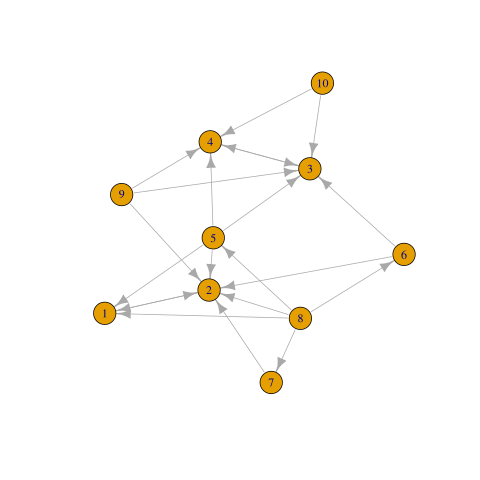
\includegraphics[width=.9\linewidth]{media/example-graph-power-walk.png}
\end{center}

\begin{figure}[htbp]
\centering
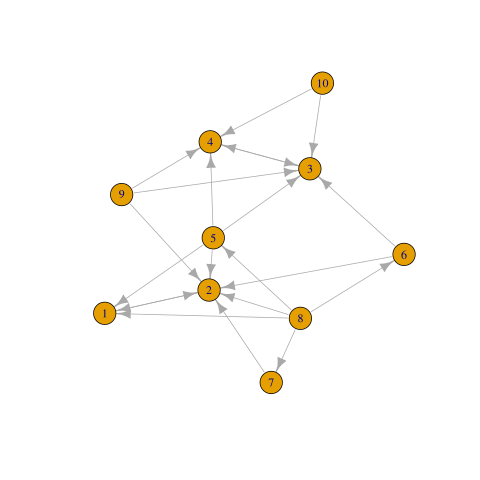
\includegraphics[width=12cm]{media/example-graph-power-walk.png}
\caption{\label{example-rs-graph}Exemplar graph for \emph{PageRank} examples, produced in listing \ref{ex-fig-r}}
\end{figure}

\subsection{Implementing the Random Surfer}
\label{sec:orgb07a4fe}
\subsubsection{Ordinary Matrices}
\label{implementing-page-rank-methods}
\paragraph{Adjacency Matrix}
\label{adjacency-matrix}
The adjacency Matrix is given by:

\begin{listing}[htbp]
\begin{minted}[]{r}
  A <- igraph::get.adjacency(g1, names = TRUE, sparse = FALSE)

  ## igraph gives back the transpose
  (A <- t(A))
\end{minted}
\caption{\label{adj-mat-random-surf}Return the Adjacency Matrix corresponding to figure \ref{example-rs-graph}}
\end{listing}

\begin{verbatim}
   1 2 8 5 7 6 9 3 4 10
1  0 1 1 1 0 0 0 0 0  0
2  1 0 1 1 1 1 1 0 0  0
8  0 0 0 0 0 0 0 0 0  0
5  0 0 1 0 0 0 0 0 0  0
7  0 0 1 0 0 0 0 0 0  0
6  0 0 1 0 0 0 0 0 0  0
9  0 0 0 0 0 0 0 0 0  0
3  0 0 0 1 0 1 1 0 1  1
4  0 0 0 1 0 0 1 1 0  1
10 0 0 0 0 0 0 0 0 0  0
\end{verbatim}

\begin{verbatim}
   1 2 8 5 7 6 9 3 4 10
1  0 1 1 1 0 0 0 0 0  0
2  1 0 1 1 1 1 1 0 0  0
8  0 0 0 0 0 0 0 0 0  0
5  0 0 1 0 0 0 0 0 0  0
7  0 0 1 0 0 0 0 0 0  0
6  0 0 1 0 0 0 0 0 0  0
9  0 0 0 0 0 0 0 0 0  0
3  0 0 0 1 0 1 1 0 1  1
4  0 0 0 1 0 0 1 1 0  1
10 0 0 0 0 0 0 0 0 0  0
\end{verbatim}

\paragraph{Probability Transition Matrix}
\label{probability-transition-matrix}
The probability transition matrix is such that each column of the
initial state distribution (i.e. the transposed adjacency matrix) is
scaled to 1.

if \(\mathbf{A}\) had vertices with a 0 out-degree, the relationship in \eqref{eq:basic-trans-def} would not work, instead columns that sum to 0 would
need to be left while all other columns be divided by the column sum to get
\(\mathbf{T}\). An alternative approach using sparse matrices will be presented
below and in this case there exists corresponding \(\mathbf{T}\) that is
stochastic and so it is sufficient to use the relationship at
\eqref{eq:basic-trans-def}, this is shown in listing \ref{basic-trans-def}.

\begin{listing}[htbp]
\begin{minted}[]{r}
(T <- A %*% diag(1/colSums(A)))

\end{minted}
\caption{\label{basic-trans-def}Solve the Transition Probability Matrix by scaling each column to 1 using matrix multiplication.}
\end{listing}

\begin{verbatim}
   [,1] [,2] [,3] [,4] [,5] [,6]      [,7] [,8] [,9] [,10]
1     0    1  0.2 0.25    0  0.0 0.0000000    0    0   0.0
2     1    0  0.2 0.25    1  0.5 0.3333333    0    0   0.0
8     0    0  0.0 0.00    0  0.0 0.0000000    0    0   0.0
5     0    0  0.2 0.00    0  0.0 0.0000000    0    0   0.0
7     0    0  0.2 0.00    0  0.0 0.0000000    0    0   0.0
6     0    0  0.2 0.00    0  0.0 0.0000000    0    0   0.0
9     0    0  0.0 0.00    0  0.0 0.0000000    0    0   0.0
3     0    0  0.0 0.25    0  0.5 0.3333333    0    1   0.5
4     0    0  0.0 0.25    0  0.0 0.3333333    1    0   0.5
10    0    0  0.0 0.00    0  0.0 0.0000000    0    0   0.0
\end{verbatim}


\subparagraph{Create a Function}
\label{create-a-function}
\begin{minted}[]{r}
   adj_to_probTrans <- function(A) {
     A %*% diag(1/colSums(A))
   }

   (T <- adj_to_probTrans(A)) %>% round(2)
\end{minted}

\begin{verbatim}
   [,1] [,2] [,3] [,4] [,5] [,6] [,7] [,8] [,9] [,10]
1     0    1  0.2 0.25    0  0.0 0.00    0    0   0.0
2     1    0  0.2 0.25    1  0.5 0.33    0    0   0.0
8     0    0  0.0 0.00    0  0.0 0.00    0    0   0.0
5     0    0  0.2 0.00    0  0.0 0.00    0    0   0.0
7     0    0  0.2 0.00    0  0.0 0.00    0    0   0.0
6     0    0  0.2 0.00    0  0.0 0.00    0    0   0.0
9     0    0  0.0 0.00    0  0.0 0.00    0    0   0.0
3     0    0  0.0 0.25    0  0.5 0.33    0    1   0.5
4     0    0  0.0 0.25    0  0.0 0.33    1    0   0.5
10    0    0  0.0 0.00    0  0.0 0.00    0    0   0.0
\end{verbatim}

\begin{verbatim}
  ##    [,1] [,2] [,3] [,4] [,5] [,6] [,7] [,8] [,9] [,10]
  ## 1     0    1    0    0 0.25  0.0    0  0.2 0.00   0.0
  ## 2     1    0    0    0 0.25  0.5    1  0.2 0.33   0.0
  ## 3     0    0    0    1 0.25  0.5    0  0.0 0.33   0.5
  ## 4     0    0    1    0 0.25  0.0    0  0.0 0.33   0.5
  ## 5     0    0    0    0 0.00  0.0    0  0.2 0.00   0.0
  ## 6     0    0    0    0 0.00  0.0    0  0.2 0.00   0.0
  ## 7     0    0    0    0 0.00  0.0    0  0.2 0.00   0.0
  ## 8     0    0    0    0 0.00  0.0    0  0.0 0.00   0.0
  ## 9     0    0    0    0 0.00  0.0    0  0.0 0.00   0.0
  ## 10    0    0    0    0 0.00  0.0    0  0.0 0.00   0.0
\end{verbatim}

\paragraph{Page Rank Random Surfer}
\label{page-rank-random-surfer}
Recall from \ref{fix} the following variables of the \emph{Random Surfer} model:


\begin{align}
    \mathbf{B} &= \alpha T +  \left( 1- \alpha \right)B :\\
\ \\
    \mathbf{B}&= \begin{bmatrix}
    \frac{1}{n} & \frac{1}{n} & \ldots & \frac{1}{n} \\
    \frac{1}{n} & \frac{1}{n} & \ldots & \frac{1}{n} \\
        \vdots      & \vdots      & \ddots & \vdots  \\
    \frac{1}{n} & \frac{1}{n} & \ldots & \frac{1}{n} \\
    \end{bmatrix} \label{eq:bgval1} \\
    n&= \left| \left| V \right| \right| \\
    \alpha &\in [0,1]
\end{align}

These are
assigned to \emph{\textbf{R}} variables in listing \ref{r-var-random-surfer}.

\begin{listing}[htbp]
\begin{minted}[]{r}
  B <- matrix(rep(1/nrow(T), length.out = nrow(T)**2), nrow = nrow(T))
  l <- 0.8123456789

  (S <- l*T+(1-l)*B) %>% round(2)


\end{minted}
\caption{\label{r-var-random-surfer}Assign Random Surfer Variables, observe the unique value given to \texttt{l}, this will be relevant later.}
\end{listing}

\begin{verbatim}
   [,1] [,2] [,3] [,4] [,5] [,6] [,7] [,8] [,9] [,10]
1  0.02 0.83 0.18 0.22 0.02 0.02 0.02 0.02 0.02  0.02
2  0.83 0.02 0.18 0.22 0.83 0.42 0.29 0.02 0.02  0.02
8  0.02 0.02 0.02 0.02 0.02 0.02 0.02 0.02 0.02  0.02
5  0.02 0.02 0.18 0.02 0.02 0.02 0.02 0.02 0.02  0.02
7  0.02 0.02 0.18 0.02 0.02 0.02 0.02 0.02 0.02  0.02
6  0.02 0.02 0.18 0.02 0.02 0.02 0.02 0.02 0.02  0.02
9  0.02 0.02 0.02 0.02 0.02 0.02 0.02 0.02 0.02  0.02
3  0.02 0.02 0.02 0.22 0.02 0.42 0.29 0.02 0.83  0.42
4  0.02 0.02 0.02 0.22 0.02 0.02 0.29 0.83 0.02  0.42
10 0.02 0.02 0.02 0.02 0.02 0.02 0.02 0.02 0.02  0.02
\end{verbatim}
\subparagraph{Eigen Value Method}
\label{eigen-value-method}
The eigenvector corresponding to the the eigenvalue of 1 will be the
stationary point, this is shown in listing \ref{eigenSol-rand-surf}

\begin{listing}[htbp]
\begin{minted}[]{r}
print(eigen(S, symmetric = FALSE, only.values = TRUE)$values, 9)
print(eigen(S, symmetric = FALSE)$vectors, 3)
\end{minted}
\caption{\label{eigenSol-rand-surf}Solve the Eigen vectors and Eigen values of the transition probability matrix corresponding to the graph.}
\end{listing}

\begin{verbatim}
 [1]  1.00000000e+00+0.0000000e+00i -8.12345679e-01+0.0000000e+00i
 [3]  8.12345679e-01+0.0000000e+00i -8.12345679e-01+0.0000000e+00i
 [5]  5.81488197e-10+0.0000000e+00i -5.81487610e-10+0.0000000e+00i
 [7] -6.74980227e-16+0.0000000e+00i  3.21036747e-17+0.0000000e+00i
 [9]  1.34928172e-18+1.1137323e-17i  1.34928172e-18-1.1137323e-17i
           [,1]         [,2]         [,3]         [,4]         [,5]
 [1,] 0.4873+0i -7.07e-01+0i  5.00e-01+0i -2.07e-03+0i -6.74e-01+0i
 [2,] 0.5268+0i  7.07e-01+0i  5.00e-01+0i  2.07e-03+0i -9.62e-02+0i
 [3,] 0.0424+0i  9.09e-18+0i -3.50e-17+0i -5.05e-17+0i  1.38e-09+0i
 [4,] 0.0493+0i -1.25e-18+0i -1.65e-16+0i  4.25e-17+0i  3.85e-01+0i
 [5,] 0.0493+0i -8.30e-18+0i -3.75e-17+0i  3.71e-17+0i  3.85e-01+0i
 [6,] 0.0493+0i -8.30e-18+0i -3.75e-17+0i  9.76e-18+0i  3.85e-01+0i
 [7,] 0.0424+0i -1.32e-18+0i -3.50e-17+0i  1.60e-17+0i -3.01e-08+0i
 [8,] 0.4915+0i -2.98e-03+0i -5.00e-01+0i -7.07e-01+0i -9.62e-02+0i
 [9,] 0.4804+0i  2.98e-03+0i -5.00e-01+0i  7.07e-01+0i -2.89e-01+0i
[10,] 0.0424+0i  5.57e-18+0i -3.77e-17+0i  3.14e-18+0i -3.24e-08+0i
              [,6]         [,7]         [,8]                [,9]
 [1,]  6.74e-01+0i  6.53e-01+0i -2.15e-01+0i -2.00e-01+1.53e-01i
 [2,]  9.62e-02+0i  1.09e-01+0i -1.96e-01+0i -1.59e-01+0.00e+00i
 [3,]  1.38e-09+0i  1.42e-15+0i -2.84e-16+0i -6.73e-17+1.32e-16i
 [4,] -3.85e-01+0i -4.37e-01+0i  7.85e-01+0i  6.37e-01+0.00e+00i
 [5,] -3.85e-01+0i -3.56e-01+0i  2.81e-01+0i  2.84e-02-1.63e-01i
 [6,] -3.85e-01+0i -3.58e-01+0i -3.68e-01+0i  4.84e-02-2.68e-01i
 [7,] -3.01e-08+0i -2.63e-02+0i -2.34e-01+0i -3.47e-02+4.29e-01i
 [8,]  9.62e-02+0i  1.32e-01+0i -6.40e-02+0i -1.09e-01-2.84e-01i
 [9,]  2.89e-01+0i  3.11e-01+0i  1.20e-01+0i -1.34e-01-1.50e-01i
[10,] -3.24e-08+0i -2.82e-02+0i -1.08e-01+0i -7.64e-02+2.83e-01i
                    [,10]
 [1,] -2.00e-01-1.53e-01i
 [2,] -1.59e-01-0.00e+00i
 [3,] -6.73e-17-1.32e-16i
 [4,]  6.37e-01+0.00e+00i
 [5,]  2.84e-02+1.63e-01i
 [6,]  4.84e-02+2.68e-01i
 [7,] -3.47e-02-4.29e-01i
 [8,] -1.09e-01+2.84e-01i
 [9,] -1.34e-01+1.50e-01i
[10,] -7.64e-02-2.83e-01i
\end{verbatim}


So in this case the stationary point corresponds to the eigenvector given by:
\[
\langle -0.49, -0.53, -0.49, -0.48, -0.05, -0.05, -0.05, -0.04, -0.04, -0.04 \rangle
\]

this can be verified by using identity \eqref{eq:eigenprob}:

$$
1 \vec{p} = S\vec{p}
$$

\begin{minted}[]{r}
  (p     <- eigen(S)$values[1] * eigen(S)$vectors[,1]) %>% Re() %>%  round(2)
\end{minted}

\begin{verbatim}
[1] 0.49 0.53 0.04 0.05 0.05 0.05 0.04 0.49 0.48 0.04
\end{verbatim}


\begin{minted}[]{r}
  (p_new <- S %*% p) %>% Re()  %>% as.vector() %>% round(2)
\end{minted}

\begin{verbatim}
[1] 0.49 0.53 0.04 0.05 0.05 0.05 0.04 0.49 0.48 0.04
\end{verbatim}


However this vector does not sum to 1 so the scale should be adjusted
(for probabilities the vector should sum to 1):

\begin{minted}[]{r}
  (p_new <- p_new/sum(p_new)) %>% Re() %>% as.vector() %>% round(2)
\end{minted}

\begin{verbatim}
[1] 0.22 0.23 0.02 0.02 0.02 0.02 0.02 0.22 0.21 0.02
\end{verbatim}

\subparagraph{Power Value Method}
\label{power-value-method}
Using the power method should give the same result as the eigenvalue method, again but for scale:

\begin{minted}[]{r}
  p_new <- p_new *123456789

  while (sum(round(p, 9) != round(p_new, 9))) {
      (p     <- p_new)
      (p_new <- S %*% p)
  }

  round(Re(p_new), 2) %>% as.vector()
\end{minted}

\begin{verbatim}
[1] 26602900 28759738  2316720  2693115  2693115  2693115  2316720 26834105
[9] 26230539  2316720
\end{verbatim}


If scaled to 1 the
same value will be returned:

\begin{minted}[]{r}
  (p_new <- p_new/sum(p_new)) %>% Re %>% as.vector() %>% round(2)
\end{minted}

\begin{verbatim}
[1] 0.22 0.23 0.02 0.02 0.02 0.02 0.02 0.22 0.21 0.02
\end{verbatim}

\subparagraph{Scaling}
\label{scaling}
If the initial state sums to 1, then the scale of the stationary
vector will also sum to 1, so this isn't in practice an issue for the power method:

\begin{minted}[]{r}
  p     <- c(1, 0, 0, 0, 0, 0, 0, 0, 0, 0)
  p_new <- S %*% p

  while (sum(round(p, 9) != round(p_new, 9))) {
      (p     <- p_new)
      (p_new <- S %*% p)
  }

  cbind(p_new, p)
\end{minted}

\begin{verbatim}
         [,1]       [,2]
1  0.21548349 0.21548349
2  0.23295388 0.23295388
8  0.01876543 0.01876543
5  0.02181424 0.02181424
7  0.02181424 0.02181424
6  0.02181424 0.02181424
9  0.01876543 0.01876543
3  0.21735625 0.21735625
4  0.21246737 0.21246737
10 0.01876543 0.01876543
\end{verbatim}

\subsubsection{Sparse Matrices}
\label{sec:orgbc96b95}
\paragraph{Creating the Probability Transition Matrix}
\label{sec:org56f48ef}
Implementing the page rank method on a larger graph requires the use of more
efficient form of matrix storage as discussed at \ref{sparse-matrix}

A sparse matrix can be created using the following syntax, which will return a
matrix of the class \texttt{dgCMatrix}:

\begin{minted}[]{r}
library(Matrix)
## Create Example Matrix
n <- 20
m <- 10^6
i <- sample(1:m, size = n); j <- sample(1:m, size = n); x <- rpois(n, lambda = 90)
A <- sparseMatrix(i, j, x = x, dims = c(m, m))

summary(A)
\end{minted}

\begin{verbatim}
1000000 x 1000000 sparse Matrix of class "dgCMatrix", with 20 entries
        i      j   x
1  832961  14530  77
2  410264  57606  97
3  782033 111998  86
4   82383 176945  93
5  110039 239517 103
6  713327 249015  98
7    3377 387382  87
8  183673 466594  90
9  459326 509037  98
10 360156 554024  91
11 697837 573216 106
12 460554 582729  80
13 353957 654474  87
14 941579 683010 108
15 955791 763690 104
16 726278 790608  85
17 317527 867693  90
18  71267 949427  81
19 126551 992218  96
20 723320 992960  84
\end{verbatim}

As before in section \ref{probability-transition-matrix}, the probability transition matrix can be found by:

\begin{enumerate}
\item Creating adjacency matrix
\begin{enumerate}
\item Transposing as necessary such that \(\mathbf{A}_{i,j}\neq 0\) indicates that \(j\) is connected to \(i\) by a directed edge.
\end{enumerate}
\item Scaling the columns to one
\end{enumerate}

To implement this for a sparseMatrix of the class \texttt{dgCMatrix}, the same
technique of multiplying by a diagonalised matrix as in \eqref{eq:diagScaleDef} may be
implemented, using sparse matrices has the advantage however that only non-zero
elements will be operated on, meaning that columns that some to zero can still
be used to create a probability transition matrix \footnote{Although this matrix may
still have columns that sum to zero and will hence be non-stochastic}
pracice an error however to create this new matrix, a new \texttt{sparseMatrix} will
need to be created using the properties of the original matrix, this can be done
like so:

\begin{listing}[htbp]
\begin{minted}[]{r}
 sparse_diag <- function(mat) {

  ## Get the Dimensions
  n <- nrow(mat)

  ## Make a Diagonal Matrix of Column Sums
  D <- sparseMatrix(i = 1:n, j = 1:n, x = colSums(mat), dims = c(n,n))

  ## Throw away explicit Zeroes
  D <- drop0(D)

  ## Inverse the Values
  D@x <- 1/D@x

  ## Return the Diagonal Matrix
  return(D)
}
\end{minted}
\caption{\label{sparse-diag}A function that takes in a column \(\rightarrow\) row adjacency matrix (\(\mathbf{A}\)) and returns a diagonal matrix (\(\mathbf{D}^{-1}_{\mathbf{A}}}\)) such that \(\vec{1}\mathbf{A} \mathbf{D}^{-1}_{\mathbf{A}} = \vec{1}\)}
\end{listing}

Applying this to the previously created sparse matrix:

\begin{minted}[]{r}
D <- sparse_diag(t(A))
summary(D)
\end{minted}

\begin{verbatim}
1000000 x 1000000 sparse Matrix of class "dgCMatrix", with 20 entries
        i      j           x
1    3377   3377 0.011494253
2   71267  71267 0.012345679
3   82383  82383 0.010752688
4  110039 110039 0.009708738
5  126551 126551 0.010416667
6  183673 183673 0.011111111
7  317527 317527 0.011111111
8  353957 353957 0.011494253
9  360156 360156 0.010989011
10 410264 410264 0.010309278
11 459326 459326 0.010204082
12 460554 460554 0.012500000
13 697837 697837 0.009433962
14 713327 713327 0.010204082
15 723320 723320 0.011904762
16 726278 726278 0.011764706
17 782033 782033 0.011627907
18 832961 832961 0.012987013
19 941579 941579 0.009259259
20 955791 955791 0.009615385
\end{verbatim}

and hence the probability transition matrix may be implemented by performing matrix multiplication accordingly:

\begin{minted}[]{r}
summary((T <- t(A) %*% D))
\end{minted}

\begin{verbatim}
1000000 x 1000000 sparse Matrix of class "dgCMatrix", with 20 entries
        i      j x
1  387382   3377 1
2  949427  71267 1
3  176945  82383 1
4  239517 110039 1
5  992218 126551 1
6  466594 183673 1
7  867693 317527 1
8  654474 353957 1
9  554024 360156 1
10  57606 410264 1
11 509037 459326 1
12 582729 460554 1
13 573216 697837 1
14 249015 713327 1
15 992960 723320 1
16 790608 726278 1
17 111998 782033 1
18  14530 832961 1
19 683010 941579 1
20 763690 955791 1
\end{verbatim}

\paragraph{Solving the Random Surfer via the Power Method}
\label{random-surfer-sparse-fix}
Solving the eigenvalues for such a large matrix will not feasible, instead the power method will need to be used to find the stationary point.

However, creating a matrix of background probabilites (denoted by \texttt{B} in section \ref{page-rank-random-surfer}) will not be feasible, it would simply be too large, instead some algebra can be used to reduce \(B\) from a matrix into a vector containing only \(\frac{1-\alpha}{N}\).

The power method is given by:

\begin{align}
\vec{p}= \mathbf{S} \vec{p}
\end{align}

where:

\begin{align}
S &= \alpha \mathbf{T} +  \left( 1 - \alpha \right) \mathbf{B} \\
\vec{p} &= \left( \alpha \mathbf{T} +  \left( 1 - \alpha \right) \mathbf{B} \right) \vec{p}\\
&= \alpha \mathbf{T}\vec{p} +  \left( 1-\alpha \right) \mathbf{B} \vec{p}
\end{align}

Let \(\mathbf{F}= \mathbf{B}\vec{p}\), consider the value of \(\mathbf{F}\) :

\begin{align}
\mathbf{F} &=
\begin{bmatrix}
\frac{1}{N} & \frac{1}{N} & \ldots & \frac{1}{N} \\
\frac{1}{N} & \frac{1}{N} & \ldots & \frac{1}{N} \\
\vdots      & \vdots      & \ddots & \vdots \\
\frac{1}{N} & \frac{1}{N} & \ldots & \frac{1}{N} \\
\end{bmatrix} \label{eq:bgVal2}
\begin{bmatrix}
\vec{p_1} \\ \vec{p_2} \\ \vdots \\ \vec{p_m}
\end{bmatrix}  \\
&= \begin{bmatrix}
\left( \sum^{m}_{i= 0}   \left[ p_i \right]  \right) \times \frac{1}{N} \\
\left( \sum^{m}_{i= 0}   \left[ p_i \right]  \right) \times \frac{1}{N} \\
\vdots  \\
\left( \sum^{m}_{i= 0}   \left[ p_i \right]  \right) \times \frac{1}{N} \\
\end{bmatrix}  \\
& \text{Probabilities sum to 1 and hence:} \\
&= \begin{bmatrix}
\frac{1}{N} \\
\frac{1}{N} \\
\frac{1}{N} \\
\vdots  \\
\frac{1}{N} \\
\end{bmatrix}
\end{align}
So instead the power method can be implemented by performing an algorithm that involves only sparse matrices:

\begin{minted}[]{r}
## Find Stationary point of random surfer
N     <- nrow(A)
alpha <- 0.85
F     <- rep((1-alpha)/N, nrow(A))  ## A nx1 vector of (1-alpha)/N

## Solve using the power method
p     <- rep(0, length.out = ncol(T)); p[1] <- 1
p_new <- alpha*T %*% p + F

## use a Counter to debug
i <- 0
while (sum(round(p, 9) != round(p_new, 9))) {
    p     <- p_new
    p_new <- alpha*T %*% p + F
    (i <- i+1) %>% print()
}

p %>% head() %>% print()
\end{minted}

\begin{verbatim}
[1] 1
[1] 2
6 x 1 Matrix of class "dgeMatrix"
        [,1]
[1,] 1.5e-07
[2,] 1.5e-07
[3,] 1.5e-07
[4,] 1.5e-07
[5,] 1.5e-07
[6,] 1.5e-07
\end{verbatim}

\subsection{Power Walk Method}
\label{sec:orga2f2c53}
Recall from \ref{pwalk} that the power walk is given by:

\begin{align*}
\mathbf{T} &= \mathbf{B} \mathbf{D}^{-1}_{B}
\end{align*}
\subsubsection{Ordinary Matrices}
\label{sec:orgd273cf2}
Implementing the Power walk using ordinary matrices is very similar to the \emph{Random Surfer} model be done pretty much the same as it is with the random surfer, but doing it with Sparse Matrices is a bit trickier.

Create the Adjacency Matrix
\begin{minted}[]{r}
  A <- igraph::get.adjacency(g1, names = TRUE, sparse = FALSE)

## * Function to create Prob Trans Mat
adj_to_probTrans <- function(A, beta) {
    B     <- A
    B     <- beta^A           # Element Wise exponentiation
    D     <- diag(colSums(B)) # B is completely dense so D ≄ 0
    D_in  <- solve(D)         # Solve returns inverse of matrix
    W     <- B %*% D_in

    return(as.matrix(W))
}

beta <- β <- 0.867
(W <- adj_to_probTrans(A, beta = β)) %>% round(2)
\end{minted}

\begin{verbatim}
   [,1] [,2] [,3] [,4] [,5] [,6] [,7] [,8] [,9] [,10]
1  0.10 0.09  0.1 0.10 0.10 0.10  0.1 0.11 0.11   0.1
2  0.09 0.11  0.1 0.10 0.10 0.10  0.1 0.11 0.11   0.1
8  0.09 0.09  0.1 0.09 0.09 0.09  0.1 0.11 0.11   0.1
5  0.09 0.09  0.1 0.10 0.10 0.10  0.1 0.09 0.09   0.1
7  0.10 0.09  0.1 0.10 0.10 0.10  0.1 0.11 0.11   0.1
6  0.10 0.09  0.1 0.10 0.10 0.10  0.1 0.09 0.11   0.1
9  0.10 0.09  0.1 0.10 0.10 0.10  0.1 0.09 0.09   0.1
3  0.10 0.11  0.1 0.10 0.10 0.10  0.1 0.11 0.09   0.1
4  0.10 0.11  0.1 0.10 0.10 0.10  0.1 0.09 0.11   0.1
10 0.10 0.11  0.1 0.10 0.10 0.10  0.1 0.09 0.09   0.1
\end{verbatim}

Look at the Eigenvalues:
\begin{minted}[]{r}
eigen(W, only.values = TRUE)$values %>% round(9)
eigen(W)$vectors/sum(eigen(W)$vectors)
\end{minted}

\begin{verbatim}
 [1]  1.000000000+0.000000000i  0.014269902+0.000000000i
 [3] -0.014148391+0.000000000i  0.014147087+0.000000000i
 [5]  0.007672842+0.004095136i  0.007672842-0.004095136i
 [7]  0.000000000+0.000000000i  0.000000000+0.000000000i
 [9]  0.000000000+0.000000000i  0.000000000+0.000000000i
               [,1]             [,2]            [,3]            [,4]
 [1,] 0.10153165+0i  5.107247e-02+0i  0.073531664+0i  0.009918277+0i
 [2,] 0.10159353+0i -1.161249e-01+0i  0.071987451+0i -0.009531974+0i
 [3,] 0.09609664+0i -2.162636e-01+0i  0.198568750+0i  0.141245296+0i
 [4,] 0.09725145+0i  6.794340e-02+0i -0.012230606+0i -0.001148014+0i
 [5,] 0.10153165+0i  5.107247e-02+0i  0.073531664+0i  0.009918277+0i
 [6,] 0.10008449+0i  1.115133e-01+0i -0.005625969+0i -0.156796770+0i
 [7,] 0.09865794+0i  1.175228e-01+0i -0.084225633+0i  0.008563891+0i
 [8,] 0.10157348+0i -6.053608e-02+0i -0.078607240+0i  0.165540590+0i
 [9,] 0.10155286+0i -6.104664e-03+0i -0.079165209+0i -0.166535117+0i
[10,] 0.10012631+0i -9.522175e-05+0i -0.157764873+0i -0.001174456+0i
                         [,5]                    [,6]             [,7]
 [1,]  0.00633946+0.04208220i  0.00633946-0.04208220i  3.014602e-16+0i
 [2,]  0.00757768+0.03910216i  0.00757768-0.03910216i  1.909248e-16+0i
 [3,]  0.22697603+0.00000000i  0.22697603+0.00000000i  3.985744e-02+0i
 [4,] -0.11628681-0.11808928i -0.11628681+0.11808928i -2.471407e-01+0i
 [5,]  0.00633946+0.04208220i  0.00633946-0.04208220i  7.520823e-02+0i
 [6,] -0.03494625-0.01031801i -0.03494625+0.01031801i  1.719325e-01+0i
 [7,] -0.07581902-0.06371153i -0.07581902+0.06371153i  6.131013e-03+0i
 [8,]  0.00717270+0.04008639i  0.00717270-0.04008639i  5.526770e-17+0i
 [9,]  0.00675977+0.04107970i  0.00675977-0.04107970i  1.105354e-16+0i
[10,] -0.03411300-0.01231382i -0.03411300+0.01231382i -4.598845e-02+0i
                  [,8]             [,9]            [,10]
 [1,] -1.791605e-17+0i -4.365749e-17+0i  1.179767e-17+0i
 [2,] -7.334385e-17+0i -8.731498e-17+0i -5.190977e-17+0i
 [3,] -1.241234e-01+0i -1.401965e-01+0i -8.894098e-02+0i
 [4,]  1.691000e-01+0i  1.687523e-01+0i  1.041947e-01+0i
 [5,] -2.144546e-01+0i  2.715852e-02+0i  3.085359e-02+0i
 [6,]  4.535455e-02+0i -1.959109e-01+0i -1.350483e-01+0i
 [7,]  7.398187e-02+0i  3.163948e-02+0i -1.260060e-01+0i
 [8,]  8.062225e-17+0i  3.638124e-17+0i  5.898837e-18+0i
 [9,]  2.687408e-17+0i  3.638124e-17+0i  5.662884e-17+0i
[10,]  5.014155e-02+0i  1.085570e-01+0i  2.149470e-01+0i
\end{verbatim}

Unlike the \emph{Random Surfer} Model in listing \ref{eigenSol-rand-surf} at \ref{eigen-value-method} the relationship between the second eigenvalue and the model parameters is not as clear, this provides that the

Use the power method

\begin{minted}[]{r}
## * Power Method
p    <- rep(0, nrow(W))
p[1] <- 1
p_new    <- rep(0, nrow(W))
p_new[2]    <- 1

while (sum(round(p, 9) != round(p_new, 9))) {
    (p     <- p_new)
    (p_new <- W %*% p)
}


p %>% as.vector()
\end{minted}

\begin{verbatim}
[1] 0.10153165 0.10159353 0.09609664 0.09725145 0.10153165 0.10008449
[7] 0.09865794 0.10157348 0.10155286 0.10012631
\end{verbatim}

\subsubsection{Sparse Matrices}
\label{sec:orgdd9086e}
\paragraph{Theory; Simplifying Power Walk to be solved with Sparse Matrices}
\label{sec:org72b32e3}
The Random Surfer model is:

$$\begin{aligned}
    \mathbf{S} &= \alpha \mathbf{T} +  \mathbf{F}  \label{eq:sparse-RS}\end{aligned}$$

where:

\begin{itemize}
\item \(\mathbf{T}\)

\begin{itemize}
\item is an \(i \times j\) matrix that describes the probability of
travelling from vertex \(j\) to \(i\)

\begin{itemize}
\item This is transpose from the way that \texttt{igraph} produces an adjacency
matrix.
\end{itemize}
\end{itemize}

\item \(\mathbf{F} = \begin{bmatrix} \frac{1}{n} \\ \frac{1}{n} \\ \frac{1}{n} \vdots \end{bmatrix}\)
\end{itemize}

Interpreting the transition probability matrix in this way is such that
\(\mathbf{T}= \mathbf{A}\mathbf{D}^{- 1}_A\) under the following
conditions:


\begin{itemize}
\item No column of \(\mathbf{A}\) sums to zero

\begin{itemize}
\item If this does happen the question arises how to deal with
\(\mathbf{D_\mathbf{A}^{- 1}}\)

\begin{itemize}
\item I've been doing \(\mathbf{D}^{\mathrm{T}}_{\mathbf{A}, i, j} := \mathtt{diag} \left( {\frac{1}{\mathtt{colsums}\left( \mathbf{A} \right)}} \right)\)
and then replacing any \(0\) on the diagonal with 1.
\end{itemize}

\item What is done in the paper is to make another matrix \(\mathbf{Z}\)
that is filled with 0, if a column sum of \(\mathbf{A}\) adds to zero
then that column in \(\mathbf{Z}\) becomes \(\frac{1}{n}\)

\begin{itemize}
\item This has the effect of making each row identical

\item The probability of going from an orphaned vertex to any other
vertex would hence be \(\frac{1}{n}\)

\item The idea with this method is then to use
\(D_\mathbf{\left( A+Z \right)}^{- 1}\) this will be consistent with
the \emph{Random Surfer} the method using \(\mathbf{F}\) in
[[\#eq:sparse-RS][]] \eqref{eq:sparse-RS}
\end{itemize}

where each row is identical that is a 0
\end{itemize}
\end{itemize}

The way to deal with the \emph{Power Walk} is more or less the same.

observe that:

\begin{align}
   \left( \mathbf{B} = \beta^{\mathbf{A}} \right)\wedge \left( \mathbf{A}_{i, j}\right)\in \mathbb{R}  \implies  \left\lvert \mathbf{B}_{i, j} \right\rvert > 0 \quad \forall i,j>n\in \mathbb{Z}^+ \label{eq:b-is-pos}
\end{align}



Be mindful that the use of exponentiation in \eqref{eq:b-is-pos} is not an element wise
exponentiation and not an actual matrix exponential.

So if I have:

\begin{itemize}
\item \(\mathbf{O}_{i, j} := 0, \quad \forall i,j\leq n \in \mathbb{Z}^+\)

\item \(\vec{p_i}\) as the state distribution, being a vector of length \(n\)
\end{itemize}

Then It can be shown (see \eqref{eq:sparse-power-walk} at \ref{solve-background-prob-power-walk-sparse}):

\begin{align}
    \mathbf{O} \mathbf{D}_{\mathbf{B}}^{-1} \vec{p_i} &= (\overrightarrow{\delta^{{\footnotesize \tmmathbf{T}}}}
     \overrightarrow{p_i})  \vec{1}\\
& = \mathtt{repeat} \left(\vec{p} \bullet \vec{\delta^{\tiny \mathrm{T}}} \mathtt{, n} \right) \\
\end{align}



where:

\begin{itemize}
\item \(\vec{\delta_i} = \frac{1}{\mathtt{colsums} \left( \mathbf{B} \right)}\)
\begin{itemize}
\item A vector\ldots{}(\(n\times 1\) matrix)
\end{itemize}
\item[{\(\vec{1}\) }] is a vector containing all 1's
\begin{itemize}
\item A vector\ldots{}(\(n\times 1\) matrix)
\end{itemize}
\item[{\(\vec{\delta^{\mathrm{T}}}\)}] refers to the transpoxe of \(\vec{\detla}\) (\(1\times n\) matrix)
\item[{\(\vec{\delta^{\mathrm{T}}} \vec{p_{i}}\)}] is some number (because it's a dot product)
\end{itemize}

This means we can do:

\begin{align}
  \overrightarrow{p_{i + 1}} & = \mathbf{T}_{\mathrm{pw}}
  \overrightarrow{p_i}\\
& = \mathbf{BD}_{\mathbf{B}}^{- 1}
  \overrightarrow{p_i}\\
  & = \left( \mathbf{B} - \mathbf{O} + \mathbf{O} \right)
  \mathbf{D}_{\mathbf{B}}^{- 1} \overrightarrow{p_i}\\
  & = \left( \left( \mathbf{B} - \mathbf{O} \right)
  \mathbf{D}_{\mathbf{B}}^{- 1} + \mathbf{OD}_{\mathbf{B}}^{- 1} \right)
  \overrightarrow{p_i}\\
  & = \left( \mathbf{B} - \mathbf{O} \right) \mathbf{D}_{\mathbf{B}}^{- 1}
  \overrightarrow{p_i} + \mathbf{OD}_{\mathbf{B}}^{- 1} \overrightarrow{p_i}\\
  & = \left( \mathbf{B} - \mathbf{O} \right) \mathbf{D}_{\mathbf{B}}^{- 1}
  \overrightarrow{p_i} + \vec{1} (\overrightarrow{\delta^{\mathrm{T}}}
  \overrightarrow{p_i}) \\
  & = \left( \mathbf{B} - \mathbf{O} \right) \mathbf{D}_{\mathbf{B}}^{- 1}
  \overrightarrow{p_i} + \mathtt{rep} (\overrightarrow{\delta^{\mathrm{T}}}
  \overrightarrow{p_i})
\end{align}

where:


Let \((\mathbf{B}-\mathbf{O}) = \mathbf{B_{\mathbf{O}}}\):

\begin{eqnarray*}
  \overrightarrow{p_{i + 1}} & = \mathbf{B_{\mathbf{O}}} \mathbf{D}_{\mathbf{B}}^{- 1}
  \overrightarrow{p_i} + \mathtt{rep} (\overrightarrow{\delta^{\mathrm{T}}}
  \overrightarrow{p_i}) &
\end{eqnarray*}

Now solve \(\tmmathbf{D}_B^{- 1}\) in terms of \(\mathbf{B_{O}}\) :

\begin{align}
  \mathbf{B}_{\mathbf{\mathbf{O}}} = & (\mathbf{B}-\mathbf{O})\\
  \mathbf{B} = & \mathbf{B}_{\mathbf{\mathbf{O}}}
  +\mathbf{O}
\end{align}

If we have \(\delta_{\mathbf{B}}\) as the column sums of\(\tmmathbf{\Beta}\) \(\mathbf{B}\):

\begin{align}
\delta^{-1}_{\mathbf{B}} &= \vec{1}\mathbf{B} \\
&= \vec{1} \left( \mathbf{B_{O}} + \mathbf{O}\right) \\
&= \vec{1}  \mathbf{B_{O}} + \vec{1}\mathbf{O} \\
&= \vec{1} \mathbf{B_{\mathbf{O}}} + \langle n, n, n, ... n \rangle \\
&= \vec{1} \mathbf{B_{\mathbf{O}}} + \vec{1} n \\
\delta_{\mathbf{B}}&=\mathtt{1/(colSums(\mathbf{B_{O}}) + n )}
\end{align}

Then if we have \(\mathit{{\tmstrong{{\tmem{D}}}}}_{\mathit{{\tmem{{\tmstrong{B}}}}}} =
\mathtt{diag} (\delta_{\tmmathbf{B}}) \mathtt{}\):


\[ \begin{array}{lll}
     \mathit{{\tmstrong{{\tmem{D}}}}}_{\mathit{{\tmem{{\tmstrong{B}}}}}}^{- 1}
     & = & \mathrm{diag} \left( \delta^{- 1}_{\mathbf{B}} \right)\\
     & = & \mathtt{diag} \left( \mathtt{ColSums}
     (\mathtt{\tmmathbf{B}_{\tmmathbf{O}}}) + \mathtt{n}
     \right)^{\mathtt{- 1}}
   \end{array} \]

And so the the power method can be implemented using sparse matrices:

\begin{align}
\vec{p_{i+1}} = \mathrm{B_{O}} \enspace \mathrm{diag}\left( \vec{1} \mathbf{B_{O}} + \vec{1}n \right) \vec{p_{i}} + \vec{1} \vec{\delta^{\mathrm{T}}\vec{p_{i}}}
\end{align}

in terms of \textbf{\emph{R}}:

\begin{minted}[]{r}
p_new <- Bo %*% diag(colSums(B)+n) %*% p + rep(t(δ) %*% p, n)

# It would also be possible to sum the element-wise product
(t(δ) %*% p) == sum(δ * p)

# Because R treats vectors the same as a nX1 matrix we could also
# perform the dot product of the two vectors, meaning the following
# would be true in R but not true generally

(t(δ) %*% p) == (δ %*% p)
\end{minted}


\subparagraph{Solving the Background Probability}
\label{solve-background-prob-power-walk-sparse}
In this case a vertical single column matrix will represent a vector and \(\otimes\) will represent the outer product (i.e. the \emph{Kronecker Product}):



Define \(\vec{\delta}\) as the column sums of
\[\begin{aligned}
     \vec{\delta} & = \mathtt{colsum} (\text{{\bfseries{B}}})^{- 1}\\
     & = \frac{1}{\overrightarrow{1^{{\scriptsize \ensuremath{\boldsymbol{T}}}}}
     \ensuremath{\boldsymbol{B}}}
   \end{aligned}\]


Then we have:


\[ \begin{aligned}
     \mathbf{OD}_{\mathbf{B}}^{- 1} \overrightarrow{p_i} & = \left(
     \begin{array}{cccc}
       1 & 1 & 1 & \\
       1 & 1 & 1 & \ldots\\
       1 & 1 & 1 & \\
       & \vdots &  & \ddots
     \end{array} \right) \left( \begin{array}{cccc}
       \frac{1}{\delta_1} & 0 & 0 & \\
       0 & \frac{1}{\delta_2} & 0 & \ldots\\
       0 & 0 & \frac{1}{\delta_{13}} & \\
       & \vdots &  & \ddots
     \end{array} \right) \left( \begin{array}{c}
       p_{i, 1}\\
       p_{i, 2}\\
       p_{i, 3}\\
       \vdots
     \end{array} \right) \nonumber \nonumber\\
     & = \left( \begin{array}{cccccc}
       \frac{p_{i, 1}}{\delta 1} & + & \frac{p_{i, 2}}{\delta_2} & + &
       \frac{p_{i, 3}}{\delta_3} & \\
       \frac{p_{i, 1}}{\delta 1} & + & \frac{p_{i, 2}}{\delta_2} & + &
       \frac{p_{i, 3}}{\delta_3} & \ldots\\
       \frac{p_{i, 1}}{\delta 1} & + & \frac{p_{i, 2}}{\delta_2} & + &
       \frac{p_{i, 3}}{\delta_3} & \\
       &  & \vdots &  &  & \ddots
     \end{array} \right) \nonumber \nonumber\\
     & = \left( \begin{array}{c}
       \sum^n_{k = 1} [p_{i, k} \delta_i]\\
       \sum^n_{k = 1} [p_{i, k} \delta_i]\\
       \sum^n_{k = 1} [p_{i, k} \delta_i]\\
       \vdots
     \end{array} \right) \nonumber\\
     & = \left( \begin{array}{c}
       \overrightarrow{\delta^{{\footnotesize \tmmathbf{T}}}}
       \overrightarrow{p_i}\\
       \overrightarrow{\delta^{{\footnotesize \tmmathbf{T}}}} \vec{p}_i\\
       \overrightarrow{\delta^{{\footnotesize \tmmathbf{T}}}} \vec{p}_i\\
       \vdots
     \end{array} \right) \nonumber\\
     & = \overrightarrow{\delta^{{\footnotesize \tmmathbf{T}}}}
     \overrightarrow{p_i} \left( \begin{array}{c}
       1\\
       1\\
       1\\
       \vdots
     \end{array} \right) \nonumber\\
     & = (\overrightarrow{\delta^{{\footnotesize \tmmathbf{T}}}}
     \overrightarrow{p_i})  \vec{1}\\
     & = \mathtt{repeat} (\overrightarrow{\delta} \overrightarrow{p_i}
     \mathtt{, n}) \label{eq:sparse-power-walk}
   \end{aligned} \]
Observe also that If we let \(\vec{\delta}\) and \(p_i\) be 1 dimensional
vectors, this can also be expressed as a dot product:

\begin{center}
\begin{tabular}{ll}
Matrices & Vectors\\
\(\vec{\delta^{\mathrm{T}}} \vec{p_{i}}\) & \(\vec{\delta} \vec{p_{i}}\)\\
\end{tabular}

\end{center}

\paragraph{Practical; Implementing the Power Walk on Sparse Matrices}
\label{sec:orgb9699b6}
\subparagraph{Inspect the newly created matrix and create constants}
\label{sec:org1d3e722}
\subparagraph{Setup}
\label{sec:org0fac7c7}
\begin{enumerate}
\item Define function to create DiagonalsSparse Diagonal Function
\label{sec:orgfc05e29}

Unlike the Random Surfer model the diagonal scaling matrix will always be given by  \(\mathbf{D}_{B}^{-1} = \mathbf{B} \enspace \mathrm{diag}\left( \frac{1}{\vec{1}\mathbf{B}}\right)\) because \(\beta^{\mathbf{A}_{i,j}} \neq 0 \quad \forall \mathbf{A}_{i,j}\), this is convenient but in any case the \texttt{sparse\_diag} function in listing \ref{sparse-diag} will still work.
\end{enumerate}

\subparagraph{Power Walk}
\label{sec:org59e0ba4}
\begin{enumerate}
\item Define B
\label{sec:orgfa96b77}
\begin{minted}[]{r}
A      <- Matrix::Matrix(A, sparse = TRUE)
B      <- A
B@x    <- β^(A@x)
B      <- A
B       <- β^A

Bo     <- A

# These two approaches are equivalent
Bo@x   <- β^(A@x) -1   # This in theory would be faster
# Bo     <- β^(A) -1
# Bo     <- drop0(Bo)


 n <- nrow(A)
\end{minted}

\begin{verbatim}
10 x 10 sparse Matrix of class "dgCMatrix"
   [[ suppressing 10 column names ‘1’, ‘2’, ‘8’ ... ]]

1  . 1 . . . . . . . .
2  1 . . . . . . . . .
8  1 1 . 1 1 1 . . . .
5  1 1 . . . . . 1 1 .
7  . 1 . . . . . . . .
6  . 1 . . . . . 1 . .
9  . 1 . . . . . 1 1 .
3  . . . . . . . . 1 .
4  . . . . . . . 1 . .
10 . . . . . . . 1 1 .
\end{verbatim}

\begin{minted}[]{r}
print(round(B, 2))
\end{minted}

\begin{verbatim}
10 x 10 Matrix of class "dgeMatrix"
      1    2 8    5    7    6 9    3    4 10
1  1.00 0.87 1 1.00 1.00 1.00 1 1.00 1.00  1
2  0.87 1.00 1 1.00 1.00 1.00 1 1.00 1.00  1
8  0.87 0.87 1 0.87 0.87 0.87 1 1.00 1.00  1
5  0.87 0.87 1 1.00 1.00 1.00 1 0.87 0.87  1
7  1.00 0.87 1 1.00 1.00 1.00 1 1.00 1.00  1
6  1.00 0.87 1 1.00 1.00 1.00 1 0.87 1.00  1
9  1.00 0.87 1 1.00 1.00 1.00 1 0.87 0.87  1
3  1.00 1.00 1 1.00 1.00 1.00 1 1.00 0.87  1
4  1.00 1.00 1 1.00 1.00 1.00 1 0.87 1.00  1
10 1.00 1.00 1 1.00 1.00 1.00 1 0.87 0.87  1
\end{verbatim}


\begin{minted}[]{r}
print(Bo,2)
\end{minted}

\begin{verbatim}
10 x 10 sparse Matrix of class "dgCMatrix"
   [[ suppressing 10 column names ‘1’, ‘2’, ‘8’ ... ]]

1  .     -0.13 . .     .     .     . .     .     .
2  -0.13 .     . .     .     .     . .     .     .
8  -0.13 -0.13 . -0.13 -0.13 -0.13 . .     .     .
5  -0.13 -0.13 . .     .     .     . -0.13 -0.13 .
7  .     -0.13 . .     .     .     . .     .     .
6  .     -0.13 . .     .     .     . -0.13 .     .
9  .     -0.13 . .     .     .     . -0.13 -0.13 .
3  .     .     . .     .     .     . .     -0.13 .
4  .     .     . .     .     .     . -0.13 .     .
10 .     .     . .     .     .     . -0.13 -0.13 .
\end{verbatim}

\item Solve the Scaling Matrix
\label{sec:org70c947d}
We don't need to worry about any terms of \(\delta_{\mathbf{B}} = \mathtt{colsums\left(B\_o\right)+n}\) being 0:

\begin{minted}[]{r}
(δB   <- 1/(colSums(Bo)+n))
\end{minted}

\begin{verbatim}
        1         2         8         5         7         6         9         3
0.1041558 0.1086720 0.1000000 0.1013479 0.1013479 0.1013479 0.1000000 0.1071237
        4        10
0.1056189 0.1000000
\end{verbatim}


\begin{minted}[]{r}
(δB   <- 1/(colSums(B)))
\end{minted}

\begin{verbatim}
        1         2         8         5         7         6         9         3
0.1041558 0.1086720 0.1000000 0.1013479 0.1013479 0.1013479 0.1000000 0.1071237
        4        10
0.1056189 0.1000000
\end{verbatim}


\item Find the Transition Probability Matrix
\label{sec:org27a8d24}
\begin{minted}[]{r}
  DB   <- diag(δB)
## ** Create the Transition Probability Matrix
## Create the Trans Prob Mat using Power Walk
  T <- Bo %*% DB
\end{minted}

\item Implement the Loop
\label{sec:org71d1ede}
\begin{minted}[]{r}
## ** Implement the Power Walk
## *** Set Initial Values
  p_new  <- rep(1/n, n)  # Uniform
  p      <- rep(0, n)    # Zero
  η      <- 10^(-6)
## *** Implement the Loop

 while (sum(abs(p_new - p)) > η) {
    (p <- as.vector(p_new)) # P should remain a vector
    sum(p <- as.vector(p_new)) # P should remain a vector
     p_new  <- T %*% p + rep(t(δB) %*% p, n)
  }
## ** Report the Values
print(paste("The stationary point is"))
print(p)
\end{minted}
\end{enumerate}

\section{Creating a Package}
\label{create-package}
In order to investigate the effect of the model parameters on the second
Eigenvalue it will be necessary to use these functions, in order to document and
work with them in a modular way they were placed into an \textbf{\emph{R}} package and made
available on \emph{GitHub} [fn: \url{https://github.com/RyanGreenup/PageRank}], to load this package use the \texttt{devtools} library as shown in listing .

\begin{listing}[htbp]
\begin{minted}[]{r}
library(devtools)
library(Matrix)
library(tidyverse) # Maybe, TODO check if this is used, I don't think it is

  if (require("PageRank")) {
      library(PageRank)
    }else{
      devtools::install_github("ryangreenup/PageRank")
      library(PageRank)
    }

\end{minted}
\caption{\label{}Load the \emph{PageRank} package which consists of the functions from \ref{implement_models}}
\end{listing}

\begin{verbatim}
Loading required package: usethis
Loading required package: PageRank

Attaching package: ‘PageRank’
\end{verbatim}


\part{Investigating \(\xi_{2}\)}
\section{Erdos Renyi Graphs}
\label{second-eigenvalue}
\subsection{ER Graphs Plotting Various Values}
\label{sec:org8c21a46}
\subsubsection{Erdos Reny Game}
\label{sec:org2144bbe}
The \emph{Erdos Renyi} game, first published in 1959 \cite{renyiRandomGraphs1959} creates a graph by assuming that the number of nodes is constant and the probability of interlinking these nodes is equal.

This is implemented in \textbf{\emph{R}} \cite[IgraphManualPagesa]{IgraphManualPages}

The Erdos Renyi game does not produce graphs consistent with networks such as
the web (see \ref{barabassi-albert}) or wikis, however, Sampling these graphs will
provide a broader picture for the overall behaviour of \(\xi_{2}\) over a broad
range of graphs with respect to the parameters of the \emph{Power Walk} method.

\subsubsection{Correlation Plot}
\label{sec:org2b2e470}

By looping over many random graphs for a variety of probabilities a data set can
be constructed and a correlation plot generated. To implement this a data frame
of input values was constructed in listing \ref{input_var}, a function that builds a
data frame with the second eigenvalue, density, determinant and trace was constructed in listing \ref{output_def} and finally a correlation plot was generated in listing \ref{corrplot} shown in figure .


\begin{listing}[htbp]
\begin{minted}[]{r}
# Generate Constants
n         <- 20
p         <- 1:n/n
beta      <- 1:n/n
beta      <- runif(n)*100
#sz       <- 1:n/n+10
sz        <- (1:n/n)*100+10
input_var <- expand.grid("n" = n, "p" = p, "beta" = beta, "size" = sz)

# Print out a sample of all the rows
input_var[sample(1:nrow(input_var), 6),]
\end{minted}
\caption{\label{input_var}A data frame consisting of input variables to be used to generate \emph{Erdos Renyi} graphs.}
\end{listing}

\begin{verbatim}
      n    p       beta size
7154 20 0.70  0.5872766  100
4103 20 0.15 82.8545866   65
133  20 0.65 64.6700020   15
3887 20 0.35 76.8201442   60
1725 20 0.25 64.6700020   35
6071 20 0.55 26.0913073   90
\end{verbatim}


\mathrm{mean}\left(\mathbf{A}\right), \left\lvert A \right\rvert,
\mathrm{tr}\left( \mathbf{A} \right)\right\(\rangle\)$\backslash$) corresponding to the \emph{Power Walk} method using the \texttt{PageRank} package discussed at \ref{create-package}.
\begin{minted}[]{r}
random_graph <- function(n, p, beta, size) {
      g1 <- igraph::erdos.renyi.game(n = sz, p)
      A <- igraph::get.adjacency(g1) # Row to column
      A <- Matrix::t(A)

      A_dens <- mean(A)
      T      <- PageRank::power_walk_prob_trans(A)
      T_tr     <- sum(diag(T))
      e2     <- eigen(T, only.values = TRUE)$values[2] # R orders by descending magnitude
      A_det  <- det(A)
      T_det  <- det(T)
      return(c(abs(e2), A_dens, T_det, T_tr)) # A_det and T_tr are uncorrelated
}
\end{minted}

\begin{listing}[htbp]
\begin{minted}[]{r}
filename <- "erdosData.rds"

if (file.exists(filename)) {

  data <- readRDS(filename)

  } else {

# Loop over the data
nc <- length(random_graph(1, 1, 1, 1))
Y  <- matrix(ncol = nc, nrow = nrow(input_var))

for (i in 1:nrow(input_var)) {
  X <- as.vector(input_var[i,])
  Y[i,] <-  random_graph(X$n, X$p, X$beta, X$size)
}

## Remove the 0i component
if (sum(abs(Y) != abs(Re(Y))) == 0) {
  Y <- Re(Y)
}

## Clean up the data frame
Y <- as.data.frame(Y); colnames(Y) <- c("eigenvalue2", "density", "determinant", "trace")
data <- cbind(input_var, Y)
data <- data[data$density!=0,]

## Save the data
saveRDS(data, filename)
}

corrplot(cor(data), method = "ellipse", type = "lower")
\end{minted}
\caption{\label{corrplot}Produce a correlation plot Created from a dataframe constructed from the values assigned in listing \ref{input_var} by using the function defined in listing \ref{output_def}, see figure .}
\end{listing}

\begin{center}
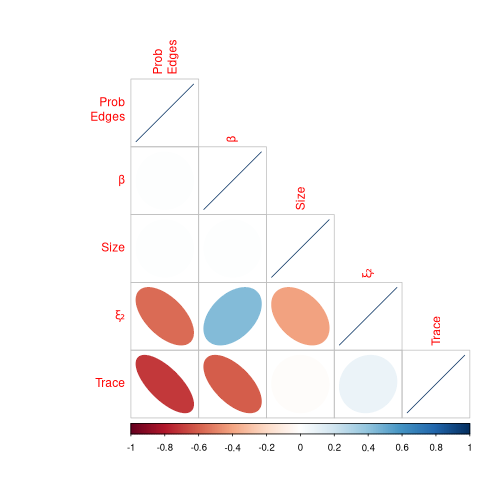
\includegraphics[width=.9\linewidth]{media/corrplot.png}
\end{center}

\subsubsection{Density of Adjacency Matrix}
\label{sec:orgf4390ce}
There appears to be a strong negative correlation between the eigenvalue and the density of the adjacency matrix.

This relationship is plotted in listing \ref{dens_plot_er} and figure \ref{fig:dens_plot_er}.

The relationship appears almost linear and so the data is log transformed and
modelled against that in listing \ref{dens_plot_er_mod} with a corresponding plot
generated in listing \ref{fig:dens_plot_er_log} and shown in figure
\ref{fig:dens_plot_er_log} revealing a concave down relationship. The quartic model
fits the data well and has the lowest \emph{MSE}, however the logarithmic model is
visually a good fit, significantly simpler and still has a low \emph{MSE}, for this
reason the logarithmic model will be used.

The coefficients of the logarithmic model, shown in listing \ref{dens_plot_er_mod}, imply the following relationship:


\begin{align}
    \xi_2 &= \left( 1-  \frac{\sum^{n}_{i= 1} \sum^{n}_{j= 1}   \mathbf{A}_{i,j}  }{n^{2}} \right)^{0.6} \cdot  e^{- 0.48} \pm \Delta
\end{align}

The maximum residual is given as 0.37 and so \(\Delta = 0.4\) would provide a
good indication for the value of the second eigenvalue by considering only the
interconnectivity of the adjacency matrix.

This suggests that a more interlinked network will converge faster when using the \emph{Power Walk} method.


\begin{listing}[htbp]
\begin{minted}[]{r}
ggplot(data) +
  geom_point(mapping = aes(x = density, y = eigenvalue2, size = beta, color = size )) +
  scale_size_continuous(range = c(0.1,1)) +
  labs(x = "Density of Adjacency Matrix", y = TeX("$\\xi_2$ of $T_{PW}$"), title = TeX("$\\xi_2$ of $T_{PW}$ given the Density of the Adjacency Matrix") ) +
  guides(size = FALSE, col = FALSE)

\end{minted}
\caption{\label{dens_plot_er}Create a Plot of \(\xi_{2}\) given Adjacency Matrix, see plot in figure \ref{fig:dens_plot_er}}
\end{listing}

\begin{figure}[htbp]
\centering
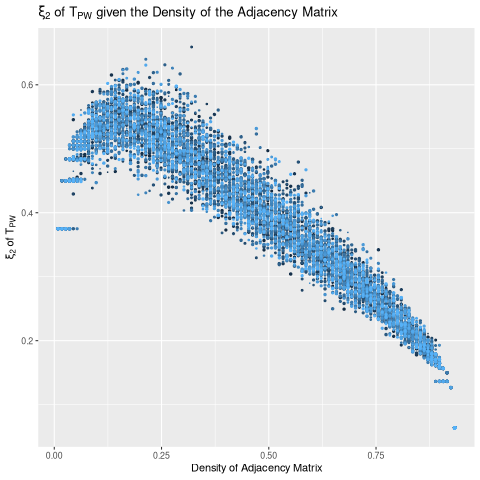
\includegraphics[width=12cm]{media/density_plot.png}
\caption{\label{fig:dens_plot_er}Plot of \(\xi_{2}\) given Adjacency Matrix, see listing \ref{dens_plot_er}}
\end{figure}


\begin{listing}[htbp]
\begin{minted}[]{r}
mod_x1 <- lm(log(eigenvalue2) ~ poly(density, 1), data = data)
data$x1 <- predict(mod_x1)

mod_x2 <- lm(log(eigenvalue2) ~ poly(density, 2), data = data)
data$x2 <- predict(mod_x2)

mod_x4 <- lm(log(eigenvalue2) ~ poly(density, 4), data = data)
data$x4 <- predict(mod_x4)

mod_xl <- lm(log(eigenvalue2) ~ log(1-density), data = data)
data$xl <- predict(mod_xl)

mod_df <- data
mod_df_long <- pivot_longer(mod_df, cols = c(x1, x2, x4, xl), names_to = "Model_Type", values_to = "eigenvalue2_mod")
mod_df_long$eigenvalue2_log <- log(mod_df_long$eigenvalue2)


print(c("MSE Linear"  = mean(mod_x1$residuals^2),
        "MSE Quadratic" = mean(mod_x2$residuals^2),
        "MSE Quartic" = mean(mod_x4$residuals^2),
        "MSE Logarithmic" = mean(mod_xl$residuals^2)
        ), 2)
cat("\n")
print(mod_xl$coefficients)
cat("\n")
print(c("Max Residual", max(mod_xl$residuals)))
\end{minted}
\caption{\label{dens_plot_er_mod}Fit Models to log transofmred Density Comparison}
\end{listing}

\begin{verbatim}
     MSE Linear   MSE Quadratic     MSE Quartic MSE Logarithmic
          0.078           0.031           0.013           0.023

     (Intercept) log(1 - density)
      -0.4798300        0.6738175

[1] "Max Residual"      "0.371075096908937"
\end{verbatim}


\begin{listing}[htbp]
\begin{minted}[]{r}
ggplot(mod_df_long, aes(x = density)) +
  geom_point(aes(y = eigenvalue2_log), fill = "lightblue", col = "black", size = 0.1, alpha = 0.2) +
  geom_smooth(aes(y = eigenvalue2_mod, col = Model_Type), size = 0.9) +
  labs(col = c("Model \nType")) +
  scale_color_discrete(labels = c("Linear", "Quadratic", "Quartic", "Logarithmic")) +
  labs(x = "Density of A", y = TeX("$ \\xi_2 $ of $\\mathbf{W}$")) +
  theme_linedraw()
\end{minted}
\caption{\label{fig:dens_plot_er_log}Plot of Log Transformed \(\xi_{2}\) against density of Adjacency matrix, using the \emph{Power Walk} algorithm applied to graphs randomly generated with the \emph{Erdos-Renyi} game.}
\end{listing}

\begin{center}
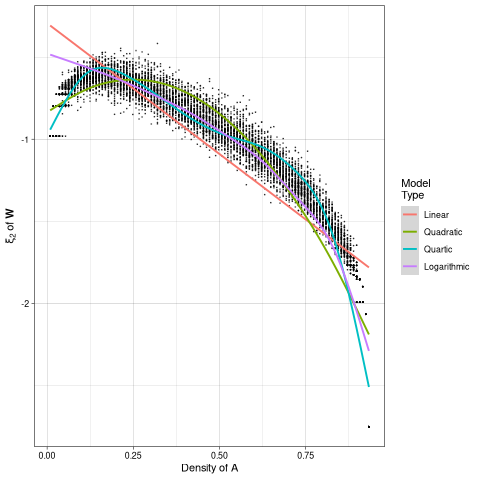
\includegraphics[width=.9\linewidth]{media/dens_plot_er_log.png}
\end{center}

\subsubsection{Trace of Transition Probability Matrix}
\label{sec:orgabb2dd7}
The correlation plot suggests that there is some positive relationship between
the trace of the transition probability matrix and the second eigenvalue, these
values are plotted in listing \ref{trace_plot_er} and figure \ref{fig:trace_plot_er}, this
relationship appears to be heteroskedastic and so it is log transformed in
listing \ref{trace_plot_log_er} and figure \ref{fig:trace_plot_log_er}. This plot is still appears to have a non constant variance but this could be due to less data corresponding to lower trace values.

The plot suggests an exponential or hyperbolic model may be a good fit, this is performed in listing \ref{mod_trace}, \ref{mod_trace_plot} and  \ref{fig:mod_trace_plot}. The hyperbolic model appears to be a reasonable fit for trace values less than half, giving the following relationship:


\begin{align}
\xi_{2} &\approx \mathrm{exp}\left( \frac{0.2}{\mathrm{tr}\left(\mathbf{T}\right)} \right) \\
	&\approx  \mathrm{exp} \left( \frac{0.2}{\mathrm{tr}\left( \mathbf{B}\mathbf{D}_{\mathbf{B}}^{- 1} \right)} \right) \label{eq:trace_lim}
\end{align}

\begin{listing}[htbp]
\begin{minted}[]{r}
ggplot(data, aes(x = trace , y = log(eigenvalue2))) +
  geom_point(mapping = aes(size = size, color = p, shape = factor(n))) +
#  stat_smooth() +
  scale_size_continuous(range = c(0.1,1.5)) +
  labs(x = "Trace of Transition Matrix", y = TeX("$\\log\\left( \\xi_2 \\right)$ of \\mathbf{W}"))
  labs(x = "Trace of Transition Matrix", y = TeX("$\\log\\left( \\xi_2 \\right)$ of \\mathbf{W}"))
\end{minted}
\caption{\label{trace_plot_log_er}Plot \(\xi_{2}\) against the trace of the matrix of the \emph{Power Walk} Transition Probability Matrix, see figure \ref{fig:trace_plot_log_er}}
\end{listing}


\begin{listing}[htbp]
\begin{minted}[]{r}
ggplot(data, aes(x = trace , y = eigenvalue2)) +
  geom_point(mapping = aes(size = size, color = p, shape = factor(n))) +
#  stat_smooth() +
  scale_size_continuous(range = c(0.1,1.5)) +
  labs(x = "Trace of Transition Matrix", y = TeX("$ \\xi_2 $ of $\\mathbf{W}$"))
\end{minted}
\caption{\label{trace_plot_er}Plot \(\xi_{2}\) against the trace of the matrix of the \emph{Power Walk} Transition Probability Matrix}
\end{listing}

\begin{figure}[htbp]
\centering
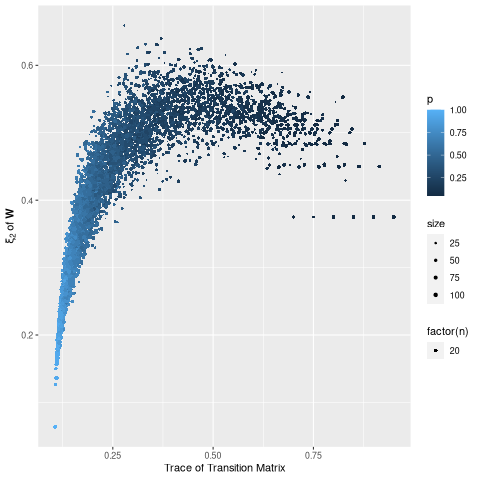
\includegraphics[width=12cm]{media/trace_plot_er.png}
\caption{\label{fig:trace_plot_er}Plot of \(\xi_{2}\) against the trace of the \emph{Power Walk} probability transition matrix}
\end{figure}


\begin{figure}[htbp]
\centering
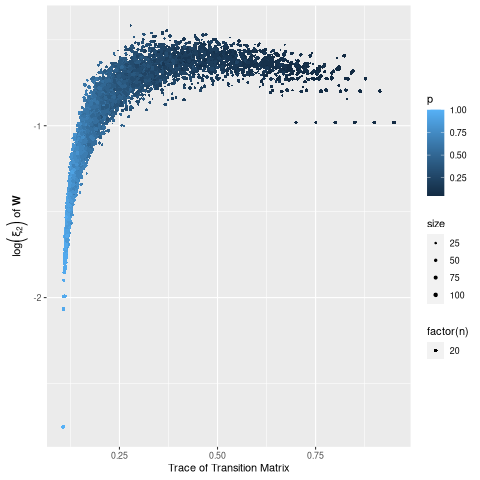
\includegraphics[width=12cm]{media/trace_plot_log_er.png}
\caption{\label{fig:trace_plot_log_er}Log transformed plot of the trace of the \emph{Power Walk} probability transition matrix}
\end{figure}

\begin{listing}[htbp]
\begin{minted}[]{r}
mod_df <- data

mod_hyp <- lm(log(eigenvalue2) ~ 0 + I(trace^(-1)), data = data)
mod_df$hyp <- predict(mod_hyp)

mod_log <- lm(log(eigenvalue2) ~ 0 + log(trace), data = data)
mod_df$log <- predict(mod_log)


mod_df_long <- pivot_longer(mod_df, cols = c(hyp, log), names_to = "Model_Type", values_to = "eigenvalue2_mod")
mod_df_long$eigenvalue2_log <- log(mod_df_long$eigenvalue2)


print(c("MSE Hyperbolic"  = mean(mod_hyp$residuals^2),
        "MSE Logarithmic" = mean(mod_log$residuals^2)), 2)
cat("\n")
print(summary(mod_hyp)$coefficients)

\end{minted}
\caption{\label{mod_trace}Fit a Hyperbolic and Logarithmic model to the data, observe that a 0 intercept is set to fix the intercept as it would be expected that a 0 trace would correspond to a 0 eigenvector, the hyperbolic model has a slightly lower mean \emph{MSE}.}
\end{listing}

\begin{verbatim}
 MSE Hyperbolic MSE Logarithmic
          0.081           0.127

                Estimate   Std. Error   t value Pr(>|t|)
I(trace^(-1)) -0.1992157 0.0005471191 -364.1176        0
\end{verbatim}


\begin{minted}[]{r}
ggplot(mod_df_long, aes(x = trace)) +
  geom_point(shape = 23, aes(y = eigenvalue2_log), fill = "lightblue", col = "black", size = 0.7, alpha = 0.4) +
  geom_line(aes(y = eigenvalue2_mod, col = Model_Type), size = 1) +
  labs(col = c("Model \nType")) +
  scale_color_manual(labels = c("Hyperbolic", "Logarithmic"),
                     values = c("indianred", "royalblue"))  +
  labs(x = "Trace of Transition Matrix", y = TeX("$\\log\\left( \\xi_2 \\right)$ of \\mathbf{W}"), title = TeX("Models Fitted to Logarithmically scaled $\\xi_{2}$ given Matrix Trace")) +
  theme_linedraw()
\end{minted}

\begin{figure}[htbp]
\centering
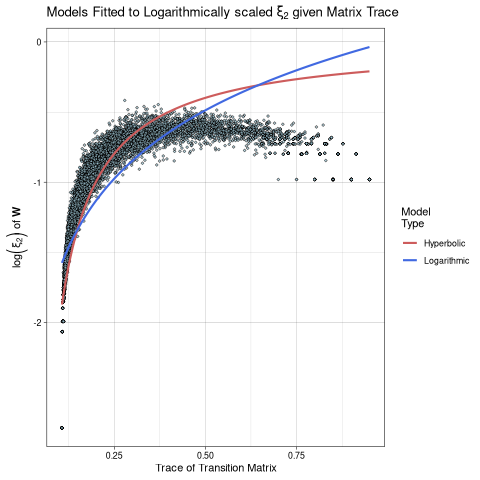
\includegraphics[width=12cm]{media/trace_models_fitted.png}
\caption{\label{fig:mod_trace_plot}Plot of the second eigenvalue logarithmically scaled across the trace of a corresponding probability transition matrix created using the \emph{Power Walk} method. The graphs were randomly generated using the \emph{Erdos Renyi} game.}
\end{figure}
\subsubsection{Conclusion}
\label{sec:orgd9803b6}
The \emph{Erdos Renyi} game produces a wide variety of all possible graphs, this provides two insights into the value of the second eigenvalue of the probability transition matrix corresponding to the power walk method:


\begin{align}
\xi_{2} &\approx  \mathrm{exp} \left( \frac{0.2}{\mathrm{tr}\left( \mathbf{B}\mathbf{D}_{\mathbf{B}}^{- 1} \right)} \right) \\
    \xi_2 &= \left( 1-  \frac{\sum^{n}_{i= 1} \sum^{n}_{j= 1}   \mathbf{A}_{i,j}  }{n^{2}} \right)^{0.6} \cdot  e^{- 0.48} \pm 0.4
\end{align}

These can be used to evaluate broadly the value of \(\xi_{2}\) and in turn the
rate of convergence of the \emph{Power Walk} method corresponding to a given graph
given only the method parameters and the adjacency matrix.

These are not however insightful of any direct relationships between the method parameters and \(\xi_{2}\), this will be considered at \ref{relate-to-random-surfer} by trying to find a relationship between the \emph{Power Walk} and the \emph{Random Surfer} models.

\subsection{Model the log transformed data using a linear regression or log(-x) regression}
\label{sec:orgbf435be}
\subsubsection{Change the colour of each model by using pivot\textsubscript{longer}}
\label{sec:org5f379a4}
\subsection{Import wikipedia data}
\label{sec:org454cea3}
\begin{itemize}
\item \sout{Import the wikipedia data}
\item \sout{Measure the density}
\item \sout{Use the density to guess the \(p\) of the game}
\begin{itemize}
\item \sout{Justify the witht the scatterplot matrix}
\end{itemize}
\item \sout{Measure the affect of different \(\beta\) values on \(\lambda_2\) for graphs ov various sizes given that \(p\) value.}
\begin{itemize}
\item \sout{Or atleast a range within that prob}

use a \emph{Barabassi-Albert} Random Graph through the \textasciitilde{}igraph::
\end{itemize}
\end{itemize}
\subsection{Look at the Trace of the Matrix as a comparison point}
\label{sec:orgbf58fe6}
\subsection{Use BA Graphs}
\label{sec:org001fdc9}

\section{Barabasi Albert Graphs}
\label{barabassi-albert}
A graph of the internet is \emph{scale free}, this means that the number of nodes of
a graph (\(n\)), having \(j\) edges is given by
 \cite[\textsection 10.7.2]{langvilleGooglePageRankScience2012}:

\begin{align}
n \propto j^{-k}, \quad \exists k \in \mathbb{R}
\end{align}

The \emph{Erdos Renyi} game is a random network, a superior approach to model the web
is to use a scale free networks \cite{barabasiPhysicsWeb2001} such as the
Barabasi-Albert graph \cite{barabasiScalefreeCharacteristicsRandom2000}

The Erdos Renyi game assumes that the number of nodes is constant from beginning
to end, clearly this is not true for networks such as the web. Consider a graph
constructed node by node where each time a new node is introduced it is randomly
connected to another with a constant probability. Despite the probability of
connecting to any given node being constant as in the Erdos Renyi game, such a
graph will favour nodes introduced earlier with respect to the number edges.
This shows that the precense of network growth is an import feature in modelling
networks.

Simply considering growth however is not sufficient to simulate graphs with a
degree distribution consistent with the web
\cite[Ch. 7]{zengPracticalSimulationMethod2013} (see figure ).

When introducing a new node, the probability of linking to any other node is not
uniformly random. When adding links to from one node to another it would be
expected that links to more popular websited would be made (for example if
somebody added a link to a personal website they might be more likely to link to
\emph{Wikipedia} than to the \emph{Encyclopedia of Britannica} simply because it is more
common). A simple approach is to presume that the probability of linking from
one node to another is proportional to the number of links, i.e. a node with
twice as many links will be twice as likely to receive a link from a new node.

These two distinguishing features departing from the \emph{Erdos Renyi} model, known as \emph{Growth} and \emph{Preferrential Attachment}, are what set the Barabassi-Albert model apart from the Erdos-Renyi model and why it is better suited to modelling networks such as the web. \cite[Ch. 7]{barabasiLinkedNewScience2002}

A practical Simulation method for social networks simulate social network links,
one possibility is \href{https://crpit.scem.westernsydney.edu.au/confpapers/CRPITV144Zeng.pdf}{this paper } \cite{zengPracticalSimulationMethod2013}.

Actually there is a data set available
 \cite{garritanoWikipediaArticleNetworks2019}, I should just analyse that, see \href{file:///home/ryan/Dropbox/DataSci/Visual\_Analytics/Assessment/the-marvel-universe-social-network/plotly3d\_Marvel.r}{how
it was done in Visual Analytics as a reminder}.


\begin{listing}[htbp]
\begin{minted}[]{r}
layout(matrix(1:2, nrow = 2))
col  <- "Mediumpurple"
n <- 1000
hist(
  igraph::degree(igraph::sample_pa(n, 0.2)),
  binwidth = 0.3,
  xlab = "",
  main = "Barabassi-Albert Degree Distribution",
  col = col, freq = FALSE
)

hist(igraph::degree(igraph::erdos.renyi.game(n, 0.2)),
     main= "Erdos-Renyi Degree Distribution",
     col = col,
     binwidth = 0.3,
     xlab = "",
     freq = FALSE )
\end{minted}
\caption{\label{degree-distribution-hist}Simulate Erdos-Renyi and Barabassi-Albert graphs in order to measure the degree distribution,  shown in \ref{fig:degree-distribution-hist}}
\end{listing}


\begin{figure}[htbp]
\centering
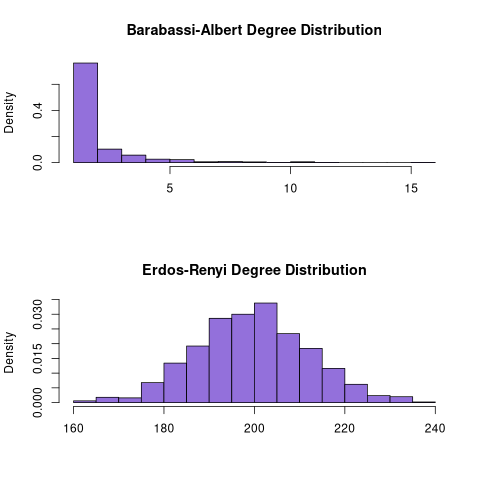
\includegraphics[width=12cm]{media/degree_dist_er_ba.png}
\caption{\label{fig:degree-distribution-hist}histograms of degree distribution of Erdos-Renyi and Barabassi-Albert graphs produced in listing \ref{degree-distribution-hist}}
\end{figure}


\section{Relating the Power Walk to the Random Surfer}
\label{relate-to-random-surfer}
\subsection{Introduction}
\label{sec:orgfca6cc6}
These are notes relating to \cite[\textsection 3.3]{parkPowerWalkRevisiting2013}, probably won't put this in the report, just arbitrary notes

So if a term in the Power Walk can be related to \(\alpha\) in the random
surfer, which is in turn \(\xi_2\), I'll be able to understand it better. \footnote{Although I'm not quite sure why \(\alpha\) is \(\xi_{2}\) either}

Consider the equation:


\begin{align*}
\mathbf{T}&= \mathbf{B}\mathbf{D}_{\mathbf{B}}^{- 1} \\
&= \left( \mathbf{B}+  \mathbf{O} - \mathbf{O} \right) \mathbf{D}_{\mathbf{B}}^{- 1} \\
\end{align*}


Break this into to terms so that we can simplify it a bit:


\begin{align*}
    \mathbf{T} &= \Bigg[ \left( \mathbf{B}- \mathbf{O} \right)\mathbf{D}_{\mathbf{B}}^{- 1} \Bigg] + \Bigg\{  \mathbf{O}\mathbf{D}_{\mathbf{B}}^{- 1} \Bigg\}
\end{align*}
\subsection{Value of [1st Term]}
\label{value-of-1st-term}
Observe that for all \(\forall i,j\in \mathbb{Z}^+\):


\begin{align*}
\mathbf{A}_{i, j} \in \left\{0, 1\right\} \\
\implies  \mathbf{B}^{\mathbf{A}_{i, j}} &\in \left\{\beta^0, \beta^1\right\} \\
                     &= \left\{1, \beta \right\}  \\
                      \implies  \beta \mathbf{A} = \left\{1, \beta \right\}
\end{align*}


Using this property we get the following


\begin{align*}
\mathbf{B}_{i,j}- \mathbf{O}_{i,j} = \left( \beta^{\mathbf{A}_{i,j}} -1 \right) &=
\begin{cases}
    0      , &\enspace \mathbf{A}_{i,j}=0  \\
    \beta-1, &\enspace \mathbf{A}_{i,j}=1  \\
\end{cases} \\
\left( \beta- 1 \right) \mathbf{A}_{i,j} &=
\begin{cases}
    0      , &\enspace \mathbf{A}_{i,j}=0  \\
    \beta-1, &\enspace \mathbf{A}_{i,j}=1  \\
\end{cases} \\
\end{align*}


This means we have


\begin{align*}
\mathbf{A} \in \left\{0, 1\right\} \forall i,j  \implies   \mathbf{B}_{i,j}- \mathbf{O}_{i,j} &= \left( \beta-1 \right) \mathbf{A}_{i,j}
\end{align*}



\begin{align*}
\mathbf{B}&= \left( \mathbf{B}+  \mathbf{O}- \mathbf{O} \right) \\
&= \left( \mathbf{B}- 1 \right)
\end{align*}

\subsection{Value of \{2nd Term\}}
\label{value-of-2nd-term}
\begin{align*}
\mathbf{O} \mathbf{D_B^{- 1}} &=
\begin{pmatrix}
    1 & 1      & 1 &        \\
    1 & 1      & 1 &\cdots  \\
    1 & 1      & 1 &        \\
      & \vdots &   &\ddots
\end{pmatrix}
\begin{pmatrix}
    \frac{1}{\delta_1} & 1                    & 1                   & \\
    1                  & \frac{1}{\delta_{2}} & 1 \cdots            & \\
    1                  & 1                    &  \frac{1}{\delta_3} & \\
               & \vdots &             &                     \ddots
\end{pmatrix}
\\
&= n
\begin{pmatrix}
    \frac{1}{n} & \frac{1}{n}      & \frac{1}{n} &        \\
    \frac{1}{n} & \frac{1}{n}      & \frac{1}{n} &\cdots  \\
    \frac{1}{n} & \frac{1}{n}      & \frac{1}{n} &        \\
      & \vdots &   &\ddots
\end{pmatrix}
\begin{pmatrix}
    \frac{1}{\delta_1} & 1                    & 1                   &        \\
    1                  & \frac{1}{\delta_2}    & 1                   & \cdots \\
    1                  & 1                    &  \frac{1}{\delta_3} &        \\
                       & \vdots               &                     & \ddots
\end{pmatrix}
\\
&= n \mathbf{E}\mathbf{D_B}^{-1}
\end{align*}


where the following definitions hold (\(\forall i, j \in \mathbb{Z}^+\)):

\begin{itemize}
\item \(\mathbf{E}_{i, j} = \frac{1}{n}\)
\item \(\mathbf{D_B}^{-1}_{k, k} = \frac{1}{\delta_k}\)
\item The value of \(\delta\) is value that each term in a column must be
divided by to become zero, in the case of the power walk that is just
\(\frac{1}{\mathtt{colSums}\left( \mathbf{B} \right)} = \vec{1}\mathbf{B}\),
but if there were zeros in a column, it would be necessary to swap out
the \$0\$s for \$1\$s and then sum in order to prevent a division by zero
issue and because the 0s should be left.
\item \(\mathbf{A}\in \left\{0, 1\right\} \forall i,j\) is the unweighted
adjacency matrix of the relevant graph.
\end{itemize}

putting this all together we can do the following:


\begin{align*}
\mathbf{T}&= \mathbf{B}\mathbf{D}^{- 1}_{\mathbf{B}} \\
&= \left( \mathbf{B}+  \mathbf{O} - \mathbf{O} \right) \mathbf{D}_{\mathbf{B}}^{- 1} \\
&= \left( \mathbf{B}- \mathbf{O} \right)\mathbf{D}_{B}^{- 1}  +  \mathbf{O} {\mathbf{D}_{\mathbf{B}}^{- 1}} \\
 \intertext{From above:} \\
&= \left( \beta- 1 \right) \mathbf{A}_{i,j} +  n \mathbf{E} \mathbf{D}_{\mathbf{B}}^{- 1}\\
&= \mathbf{A}_{i,j}\left( \beta- 1 \right)  +  n \mathbf{E} \mathbf{D}_{\mathbf{B}}^{- 1}\\
 \intertext{because $\mathbf{D} \mathbf{D}^{- 1} = \mathbf{I}$ we can multiply one side through:} \\
&= \mathbf{D}_{\mathbf{A}} \mathbf{D}_{\mathbf{A}}^{- 1}\mathbf{A}_{i,j}\left( \beta- 1 \right)  +  n \mathbf{E} \mathbf{D}_{\mathbf{B}}^{- 1}\\
\end{align*}


But the next step requires showing that:


\begin{align*}
\left( \beta-1 \right)\mathbf{D}_\mathbf{A} \mathbf{D}_{\mathbf{B}}^{- 1} &= \mathbf{I} - n \mathbf{D}_{B}^{- 1}
\end{align*}

\subsection{Equate the Power Walk to the Random Surfer}
\label{sec:org57926cf}
Define the matrix \(\mathbf{D}_{\mathbf{M}}\):

\begin{align}
    \mathbf{D}_{\mathbf{M}} = \mathrm{diag}\left( \mathtt{colSum} \left( \mathbf{M} \right) \right) &= \mathrm{diag} \left( \vec{1} \mathbf{M} \right)
\end{align}


To scale each column of that matrix to 1, each column will need to be divieded by the column sum, unless the column is already zero, this needs to be done to turn an adjacency matrix into a matrix of probabilities:

\begin{align}
    \mathbf{D}_{\mathbf{A}} ^{- 1} :  \left[     \mathbf{D}_{\mathbf{A}} ^{- 1}  \right]_i =
    \begin{cases}
	0 ,& \quad \left[ \mathbf{D}_{\mathbf{A}} \right]_i = 0 \\
	\left[ \frac{1}{\mathbf{D}_{\mathbf{A}}} \right] ,& \enspace \enspace \left[ \mathbf{D}_{\mathbf{A}} \right]_i \neq 0
    \end{cases}
\end{align}

In the case of the power walk \(\mathbf{B}= \beta^{\mathbf{A}} \neq 0\) so it is sufficient:

\begin{align}
    \mathbf{D}_{\mathbf{B}}^{- 1} &= \frac{1}{\mathrm{diag}\left( \vec{1} \left(\mathbf{\beta^{\mathbf{A}}  \right) } \right)}
\end{align}


Recall that the \emph{power walk} gives a transition probability matrix:

\begin{align}
%    \mathbf{T} &= \mathbf{a} \text{\fboxsep=.2em\fbox{$x$}} \\
    \text{\textbf{Power Walk}} \nonumber \\
\mathbf{T} &= \text{\fboxsep=.2em\fbox{$\mathbf{A}\mathbf{D}_{\mathbf{A}}^{- 1}$}}  \mathbf{D}_{\mathbf{A}} \left( \beta - 1 \right) \mathbf{D}_{\mathbf{B}}^{- 1} + \text{\fboxsep=.2em\fbox{$\mathbf{E}$}} n \mathbf{D}_{\mathbf{B}}^{- 1}  \label{eq:pwbx}\\
    \text{\textbf{Random Surfer}} \nonumber \\
    \mathbf{T} &= \alpha \text{\fboxsep=.2em\fbox{$\mathbf{A}\mathbf{D}_{\mathbf{A}}^{- 1}$}}  + \left( 1-\alpha \right) \text{\fboxsep=.2em\fbox{$\mathbf{E}$}}
\end{align}

So these are equivalent when:

\begin{align}
\mathbf{D}_{\mathbf{A}}   \left( \beta -  1 \right)\mathbf{D}_{\mathbf{B}^{- 1}} &=\mathbf{I}  \alpha \label{fl} \\
    \ \nonumber \\
  \vec{1}  \left( 1- \alpha \right) &=  - n \mathbf{D}_{\mathbf{B}}^{- 1}  \nonumber \\
    \implies  \vec{1}\alpha &=  \vec{1}- n \mathbf{D}_{\mathbf{B}}^{- 1} \label{st} \\
    \intertext{Hence we have:} \notag \\
\mathbf{D}_{\mathbf{A}}  \left( \beta -  1 \right)\mathbf{D}_{\mathbf{B}}^{- 1} &=  \vec{1}\alpha =  \mathbf{I}- n \mathbf{D}_{\mathbf{B}}^{- 1} \label{eq:eqalpha}
\end{align}


Solving for \(\beta\)  with \eqref{fl} :

\begin{align}
    \beta&= \frac{1- \Theta}{\Theta}\\
%    \beta&= \frac{\alpha - \mathbf{D}_{\mathbf{A}}\mathbf{D}_{\mathbf{B}}^{- 1}}{\mathbf{D}_{\mathbf{A}}\mathbf{D}_{\mathbf{B}}^{-1}}
\end{align}

where: \footnote{NOTE: Similar to a signmoid function, which is a solution to \(p \propto p(1-p)\), I wonder if this provides a connection to the exponential nature of the power walk
`erdos.renyi`erdos.renyi``}

\begin{itemize}
\item \(\Theta = \mathbf{D}_{\mathbf{A}} \mathbf{D}_{\mathbf{B}}^{- 1}\)
\end{itemize}

but we can't really do this so instead:

\[
\beta \mathbf{1}_{\tiny \left[ n,n \right]}  = \left( 1 - \Theta \right) \Theta^{-1} \label{eq:betadef}
\]

If \(\beta\) is set accordingly then by \eqref{eq:eqalpha}:

\begin{align}
    \mathbf{A}\left( \beta- 1 \right) \mathbf{D}_{\mathbf{B}}^{- 1} &= \alpha = \mathbf{I}- n \mathbf{D}_{\mathbf{B}}^{- 1} \nonumber \\
     \implies  \mathbf{A}\left( \beta- 1 \right) \mathbf{D}_{\mathbf{B}}^{- 1} &=  \mathbf{I}- n \mathbf{D}_{\mathbf{B}}^{- 1}
\end{align}

And setting \(\Gamma = \mathbf{I}- n \mathbf{D}_{\mathbf{B}}^{- 1}\)  from \eqref{st} and putting in \eqref{eq:pwbx} we have:

\begin{align}
\mathbf{T} &= \text{\fboxsep=.2em\fbox{$\mathbf{A}\mathbf{D}_{\mathbf{A}}^{- 1}$}}  \mathbf{D}_{\mathbf{A}} \left( \beta - 1 \right) \mathbf{D}_{\mathbf{B}}^{- 1} + \text{\fboxsep=.2em\fbox{$\mathbf{E}$}} n \mathbf{D}_{\mathbf{B}}^{- 1}  \nonumber \\
  \mathbf{T} &= \Gamma \text{\fboxsep=.2em\fbox{$\mathbf{A}\mathbf{D}_{\mathbf{A}}^{- 1}$}}  + \left( 1-\Gamma \right) \text{\fboxsep=.2em\fbox{$\mathbf{E}$}} \nonumber \\
  \ \nonumber \\
  \mathbf{T} &= \Gamma \mathbf{A}\mathbf{D}_{\mathbf{A}}^{- 1}  + \left( 1-\Gamma \right) \mathbf{E}
  \end{align}

Where \(\mathbf{E}\) is square matrix of \(\frac{1}{n}\) as in \eqref{eq:bgval1}  \eqref{eq:bgVal2}

\subsection{Conclusion}
\label{sec:org1df4dbb}
So when the adjacency matrix is stictly boolean, the power walk is equivalent to the random surfer.

\subsection{The Second Eigenvalue}
\label{sec:org3c366ba}
\subsubsection{The Random Surfer}
\label{sec:orga21618e}
The Second eigenvalue \(\xi_2\) of the Power Surfer is less than \(\alpha\) (\href{Proposal/Propsal.org}{See 3.2; Stability and Concvergence, of proposal}).
\subsubsection{Power Walk}
\label{sec:org5ff090f}
Because the Power Walk relates to the random surfer as demonstrated in section , what can be said about \(\xi_{2}\)
\paragraph{Applying this to Power Walk}
\label{sec:orge4c0b30}
Let \(\Lambda_{\left( 2 \right)}\left( \mathbf{T} \right) = \lambda_2\) return the second value of a transition, probability Matrix, then observe that:


\begin{align}
    \Lambda_{\left( 2 \right)} \left( \mathbf{T}_{\text{\tiny RS}} \right)  \leq \left\lvert \alpha \right\rvert  \implies      \Lambda_{\left( 2 \right)} \left( \mathbf{T}_{\text{\tiny PW}} \right) \leq \left\lvert \frac{\alpha - \mathbf{D}_{\mathbf{a}} \mathbf{D}_{\mathbf{B}}^{- 1}}{\mathbf{D}_{\mathbf{A}}\mathbf{D}_{\mathbf{B}}^{-1}}  \right\rvert
\end{align}

where:


\begin{itemize}
\item \(\lambda_{\left( 2 \right)} \left( \mathbf{T} \right)\) refers to the transition probability matrix of the power walk and random surfer approaces as indicated.
\end{itemize}
\subparagraph{My attempt}
\label{sec:org30e6ada}
\begin{align}
    \beta \mathbf{1}_{\tiny \left[ n, n \right] }    &= \frac{1- \Theta}{\Theta} \label{eq:betasig}\\
%    \beta&= \frac{\alpha - \mathbf{D}_{\mathbf{A}}\mathbf{D}_{\mathbf{B}}^{- 1}}{\mathbf{D}_{\mathbf{A}}\mathbf{D}_{\mathbf{B}}^{-1}}
\end{align}

where:
\begin{itemize}
\item \(\Theta = \mathbf{D}_{\mathbf{A}} \mathbf{D}_{\mathbf{B}}^{- 1}\)
\end{itemize}

So I thought maybe if I could find a value of \(\beta\) that satisfied \eqref{eq:betasig} then I could show circumstances under which \(\left\lvert \xi_2 \right\rvert < \alpha\).

Seemingly it's only satisfied where \(\beta = 1\) though, using this simulation:

\begin{minted}[]{r}
g1 <- igraph::erdos.renyi.game(n = 9, 0.2)
A <- igraph::get.adjacency(g1) # Row to column
A <- t(A)
# plot(g1)

## * Finding beta values to behave like Random Surfer
  beta <- 10
  B <- beta^A

  DA     <- PageRank::create_sparse_diag_sc_inv_mat(A)
  DB_inv <- PageRank::create_sparse_diag_scaling_mat(B)

 THETA <- DA %*% DB_inv

THETA <- function(A, beta) {
  B  <- beta^A
  DA     <- PageRank::create_sparse_diag_sc_inv_mat(A)
  DB_inv <- PageRank::create_sparse_diag_scaling_mat(B)
  return(DA %*% DB_inv)
}

THETA_inv <- function(A, beta) {
  B  <- beta^A
  DB     <- PageRank::create_sparse_diag_sc_inv_mat(B)
  DA_inv <- PageRank::create_sparse_diag_scaling_mat(A)
  return(DA %*% DB_inv)
}

beta_func <- function(A, beta) {
    return(1-THETA(A, beta^A) %*% THETA_inv(A, beta^A))
}

THETA(A, 10) %*% THETA_inv(A, 10)


eta <- 10^-6
beta <- 1.01
while (mean(beta*matrix(1, nrow(A), ncol(A)) - beta_func(A, beta)) > eta) {
    beta <- beta + 0.01
    print(beta)
    print(diag(beta_func(A, beta)))
    print(beta*matrix(1, nrow(A), ncol(A)))
    print(beta_func(A, beta))
#    Sys.sleep(0.1)
}

beta


diag(beta_func(A, beta))
beta


## * blah
\end{minted}

\section{Appendix}
\label{sec:org15bc984}

\begin{listing}[htbp]
\begin{minted}[]{r}
library(Matrix)
library(igraph)
n <- 200
m <- 5
power <- 1
g <- igraph::sample_pa(n = n, power = power, m = m, directed = FALSE)
plot(g)
A <- t(get.adjacency(g))
plot(A)
image(A)


# Create a Plotting Region
par(pty = "s", mai = c(0.1, 0.1, 0.4, 0.1))


# create the image

title=paste0("Undirected Barabassi Albert Graph with parameters:\n Power = ", power, "; size = ", n, "; Edges/step = ", round(m))
image(A, axes = FALSE, frame.plot = TRUE, main = title, xlab = "", ylab = "",  )
\end{minted}
\caption{\label{r-den_undir_ba}\textbf{\emph{R}} code to produce an image illustrating the density of a simulated Barabasi-Albert graph, the \emph{Barabasi-Albert} graph is a good analouge for the link structure of the internet \cite{langvilleGooglePageRankScience2012,barabasiPhysicsWeb2001,barabasiScalefreeCharacteristicsRandom2000} see the output in figure \ref{fig:den_undir_ba}}
\end{listing}

\begin{figure}[htbp]
\centering
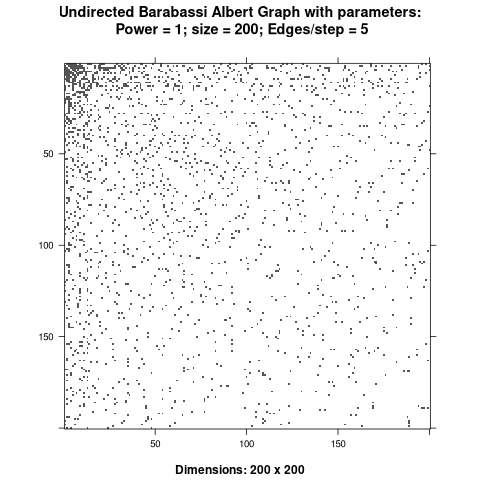
\includegraphics[width=12cm]{media/DensityUndirectedBA.png}
\caption{\label{fig:den_undir_ba}Plot of the adjacency matrix corresponding to a Barabassi-Albert (i.e. \emph{Scale Free}) Graph produced by listing \ref{r-den_undir_ba}, observe the matrix is quite sparse.}
\end{figure}
\subsection{Graph Diagrams}
\label{sec:org4d02de3}
Graph Diagrams shown in \ref{markov} where produced using \texttt{DOT} (see \cite{DOTLanguage,DOTGraphDescription2020}).
\subsection{Definitions}
\label{definitions}
The following definitions are used in this report \footnote{see generally \cite[Ch. 15]{langvilleGooglePageRankScience2012} for further reading} :

\begin{description}
\item[{Markov Chains}] are discrete mathematical model such that future values depend only on current values \cite[\textsection 1.5]{larsonElementaryLinearAlgebra1991}
\item[{Stochastic Matrices}] contain only positive values where each column sums to 1 \cite{langvilleGooglePageRankScience2012,larsonElementaryLinearAlgebra1991} (i.e. \(\mathbf{T}\) is stochastic \(\iff \vec{1}\mathbf{T} = \vec{1}\))
\begin{itemize}
\item some authors use rows (see e.g. \cite[\textsection 15.3]{langvilleGooglePageRankScience2012}), in this paper columns will be used, i.e. columns will add to one and an entry \(\mathbf{A}_{i,j} \neq 0\) will indicate that travel is permitted from vertex \(j\) to vertex \(i\).
\begin{itemize}
\item \emph{Column Stochastic} and \emph{Row Stochastic} can be used to more clearly distinguish between which type of stochastic matrix is being used.
\end{itemize}
\item Many programming languages return \emph{unit-eigenvectors} \(\vec{x}\) such that \(\left\lvert \left\lvert \vec{x} \right\rvert \right\rvert = 1\) as opposed to \(\mathtt{sum} \left( \vec{\mathtt{x}}\right) = 1\), so when solving for a stationary vector it can be necessary to perform \(\vec{\mathtt{p}} \leftarrow \frac{\vec{\mathtt{p}}}{\sum \vec{p}}\)
\end{itemize}
\item[{Irreducible}] graphs have a path from from any given vertex to another vertex. \cite[\textsection 15.2]{langvilleGooglePageRankScience2012}
\begin{description}
\item[{Ergodic}] graphs are irreducible graphs with further constraints outside
the scope of this report (see e.g.
\cite{nathanaelackermancameronfreeralexkruckmanandrehanapatelProperlyErodicStructures2017,chenEigenvaluesInequalitiesErgodic2005})
\begin{itemize}
\item It is a necessary but not a sufficient condition of ergodic graphs that all vertices be reachable from any other vertices (see \cite{sazProbabilityTheoryThis} for a counter example.)
\end{itemize}
\end{description}
\item[{Primitive Matrices}] are non-negative irreducible matrices that have only one eigenvalue on the unit circle.
\begin{itemize}
\item If a matrix is primitive it will approach a limit under exponentiation \cite[\textsection 15.2]{langvilleGooglePageRankScience2012}
\end{itemize}
\item[{Transition Probability Matrix}] is a stochastic matrix where each column is a vector of probabilities such that \(\mathbf{T}_{i,j}\) represents the probability of travelling from vertex \(j\) to vertex \(i\) during a random walk.
\begin{itemize}
\item Some Authors consider the transpose (see e.g. \cite{langvilleGooglePageRankScience2012}).
\end{itemize}
\item[{Aperiodic}] Markov chains are markov chains with an irreducible and primitive transition probability matrix.
\begin{itemize}
\item If the transition probability matrix is irreducible and imprimitive it is said to be a periodic Markov chain.
\end{itemize}
\item[{Regular}] Markov Chains are regular irreducible and aperiodic.
\item[{Sparse}] Matrices contain a majority of elements with values equal to 0 \cite[\textsection 4.2]{langvilleGooglePageRankScience2012}
\item[{Sparse}] Iterating the
\item[{PageRank}] A process of measuring graph centrality by using a random walk algorithm and measuring the most frequent node
\begin{itemize}
\item In the literature (see e.g. \cite{guptaWTFWhoFollow2013,langvilleGooglePageRankScience2012}) the Random Surfer model is usually used to refer to the introduction of a probability of travelling to any other node, this is discussed in CROSSREF
\end{itemize}
\end{description}
\subsubsection{Notation}
\label{notation}
\begin{itemize}
\item \(\mathbf{A}\)
\begin{itemize}
\item Is the adjacency matrix of a graph such that \(\mathbf{A}_{i,j} = 1\) Indicates travel from \(j\) to \(i\) is possible.
\end{itemize}
\item \(\mathbf{T}\)
\begin{itemize}
\item Indicates the probability of a movement during a random walk, such that \(\mathf{T}_{i,j}\) is equal to the probability of travelling \(j \rightarrow  i\) during a random walk.
\end{itemize}
\item \(\mathbf{D}_{\mathbf{A}}=\mathrm{diag}\left(\vec{1}\mathbf{A}\right)\)
\item \(\mathbf{D}_{\mathbf{A}}^{- 1}  =
   \begin{cases}
   0 ,& \quad \left[ \mathbf{D}_{\mathbf{A}} \right]_i = 0 \\
   \left[ \frac{1}{\mathbf{D}_{\mathbf{A}}} \right] ,& \enspace \enspace \left[ \mathbf{D}_{\mathbf{A}} \right]_i \neq 0
   \end{cases}\)
\begin{itemize}
\item A diagonal scaling matrix such that \(\mathbf{T} = \mathbf{A} \mathbf{D}_{\mathbf{A}}^{-1}\), the piecewise definition is such that \(\mathbf{D}^{-1}_{\mathbf{A}}\) is still defined even if \(\mathbf{A}\) is a reducible graph.
\begin{itemize}
\item Where \(\mathbf{D}^{-1}\) is a matrix such that multiplication with which scales each column of \(\mathbf{A}\) to 1.
\item \(\mathbf{D}^{-1}_{\mathbf{A}} = \vec{1}\mathbf{D}^{-1}_{\mathbf{A}} = \frac{1}{\vec{1}\mathbf{D}_{\mathbf{A}}}\) for some stochastic matrix \(\mathbf{A}\)
\end{itemize}
\end{itemize}
\item \(n\)
\begin{itemize}
\item Refers to the number of vertices in a graph, \(n = \mathtt{nrow}\left(\mathbf{A}\right) = \mathtt{ncol}\left(\mathbf{A}\right)\)
\end{itemize}
\item \(\mathbf{E}_{i,j} = \frac{1}{n}\)
\begin{itemize}
\item A matrix of size \(n\times n\) representing the background probability of jumping to any vertex of a graph.
\end{itemize}
\item \(\vec{1}\)
\begin{itemize}
\item a vector of length \(n\) containing only the value 1.
\begin{itemize}
\item The convention that a vector behaves as a vertical \(n \times 1\) matrix will be used here.
\item Some authors use \(\mathbf{e}\), see e.g. \cite{langvilleGooglePageRankScience2012}
\end{itemize}
\end{itemize}
\item \(\mathbf{J} = \vec{1}\cdot \vec{1}^{\mathrm{T}} \iff \mathbf{J}_{i,j} = 1\)
\begin{itemize}
\item A completely dense \(n \times n\) matrix containing only 1
\end{itemize}
\item \(\alpha\)
\begin{itemize}
\item The probability of teleporting from one vertex to another during a random walk.
\begin{itemize}
\item In the literature \(\alpha\) is often referred to as a damping factor (see e.g.  \cite{berkhoutRankingNodesGeneral2018a,brinkmeierPageRankRevisited2006a,fuDampingFactorGoogle2006,kamvarAdaptiveMethodsComputation2004b,bianchiniPageRank2005})
\end{itemize}
\end{itemize}
or a smoothing constant (see e.g \cite{koppelMeasuringDirectIndirect2014}).
\end{itemize}

\section{my to do list}
\label{sec:orga2c9e13}
\subsection{Look at the Trace of the Matrix as a comparison point}
\label{sec:orgcf2dee5}
\subsection{Use BA Graphs}
\label{sec:orgc038ea9}
**
\subsection{TODO Diamater}
\label{sec:org0e45f49}
Diamater of the web sounds like a fun read \cite{albertDiameterWorldWideWeb1999}
\subsection{Improving the Performance of Page Rank}
\label{sec:orgfd61c07}

This:

\begin{quote}
Another approach involves involves reordering the problem and taking advantage
of the fact that the transition probability matrix is sparse  in order
to produce a new algorithm which cannot perform worse than the \emph{power method}
but has been shown to improve the rate of convergence in certain cases.
\cite{langvilleReorderingPageRankProblem2006}.
\end{quote}


There was also a book that I downloaded that mentioned it

Accellerating the Computatoin of Page Rank \cite{langvilleGooglePageRankScience2012}
\end{document}
